%\documentclass[review,3p,10pt,times]{elsarticle}
\documentclass[10pt]{article}
\usepackage{a4wide} 
\usepackage{shadow}        % allows shadow boxes for figures
\usepackage{hhline}        % fancy table lines
\usepackage{tabularx}      % tables that auto-size
\usepackage{latexsym}      % make some extra symbols available
\usepackage{pslatex}       % Ensure we use non-bitmap fonts
\usepackage{fancyhdr} % Allows control of header/footer
\usepackage{graphics}
\usepackage{epsfig}
\usepackage{url}           % Properly line wraps URLs: \url{...}
\usepackage{subfigure}
\usepackage[%
  ps2pdf,              % using ps2pdf vs pdftex
  colorlinks=true,     % color the words instead of use a colored box
  urlcolor=blue,       % \href{...}{...} external (URL)
  filecolor=blue,      % \href{...} local file
  linkcolor=black,     % \ref{...} and \pageref{...}
  citecolor=black,     % \cite{}
%  pdftitle={},
%  pdfauthor={},
%  pdfsubject={},
%  pdfkeywords={},
%  pdfproducer={pdfLaTeX},
%  pagebackref,        % backward references in the bibliography
  pdfpagemode=UseOutlines,  % None, UseThumbs, UseOutlines, FullScreen
  bookmarksopen=true   % Does outline start expanded?
  ]{hyperref}
\usepackage[%
  font=small,
%  font=footnotesize,
  labelfont=bf
  ]{caption}


%-- margins
%replace setlength with renewcommand
\setlength{\headheight}{0.0in}
\setlength{\textheight}{9.0in}
\setlength{\footskip}{0.3in}
\setlength{\headsep}{0.3in}
\setlength{\topmargin}{-0.3in}
\setlength{\textwidth}{6.5in}
\setlength{\columnsep}{0.25in}
\setlength{\oddsidemargin}{0in}
\renewcommand{\baselinestretch}{2}
\evensidemargin \oddsidemargin

\setlength{\parindent}{0pc}
\setlength{\parskip}{4.5pt}


\begin{document}

%-- include the standard formatting macros... you should use these
\input{std_commands.tex}

%\begin{frontmatter}

%-- don't print date
\date{}

{
\renewcommand{\baselinestretch}{1.0}

%-- Document title and authors
\title{Applying performance models to understand data-intensive computing efficiency}

\author{\rm Elie Krevat$^\ast$, Tomer Shiran$^\ast$, Eric
Anderson$^\dagger$, Joseph Tucek$^\dagger$, Jay J. Wylie$^\dagger$, Gregory R. Ganger$^\ast$ \\
$^\ast$Carnegie Mellon University $^\dagger$HP Labs}

%\author[A]{Elie Krevat}
%\author[A]{Tomer Shiran}
%\author[B]{Eric Anderson}
%\author[B]{Joseph Tucek}
%\author[B]{Jay J. Wylie}
%\author[A]{Gregory R. Ganger}
%\address[A]{Carnegie Mellon University}
%\address[B]{HP Labs}

%\renewcommand{\headrulewidth}{0pt}
%\cfoot{}
\maketitle

%-- Use ``fancy'' to include the above Appears in... stuff
\thispagestyle{empty}
%\thispagestyle{fancy}


%-- To remove page numbers, uncomment
%\pagestyle{empty}

%-- All other files included from this one
\begin{abstract}
New programming frameworks for scale-out parallel analysis, such
as MapReduce and Hadoop, have become a cornerstone for exploiting
large datasets.  However, there has been little analysis of how these
systems perform relative to the capabilities of the hardware on which they run.
This paper describes a simple analytical model that predicts the
optimal performance of a parallel dataflow system.
The model exposes the inefficiency of popular scale-out systems,
which take 3--13$\times$ longer to complete jobs than the hardware
should allow, even in well-tuned systems used to achieve record-breaking
benchmark results.
To validate the sanity of our model, we present small-scale
experiments with Hadoop and a simplified dataflow processing tool
called Parallel DataSeries.
Parallel DataSeries achieves performance close to the analytic
optimal, showing that the model is realistic and that large improvements
in the efficiency of parallel analytics are possible.


\end{abstract}
}

%\begin{keyword}
%Cloud Computing
%\sep 
%DISC
%% PACS codes here, in the form: \PACS code \sep code

%% MSC codes here, in the form: \MSC code \sep code
%% or \MSC[2008] code \sep code (2000 is the default)

%\end{keyword}

%\end{frontmatter}

\section{Introduction}
\label{sec:intro}

%This is the introduction to the paper.  It includes a motivating graph in Figure~\ref{fig:slowdown}.

``Data-intensive scalable computing'' (DISC) refers to a rapidly growing style
of computing characterized by its reliance on huge and growing
datasets~\cite{disc}.  Driven by the desire and capability to extract
insight from such datasets, data-intensive computing is quickly
emerging as a major activity of many organizations.  With massive
amounts of data arising from such diverse sources as telescope
imagery, medical records, online transaction records, and web pages,
many researchers are discovering that statistical models extracted
from data collections promise major advances in science, health care,
business efficiencies, and information access.  Indeed, statistical
approaches are quickly bypassing expertise-based approaches in terms
of efficacy and robustness.

To assist programmers with data-intensive computing, new programming
frameworks (e.g., MapReduce~\cite{mapreduce}, Hadoop~\cite{hadoop} and
Dryad~\cite{dryad}) have been developed.  They provide abstractions
for specifying data-parallel computations, and they also provide
environments for automating the execution of data-parallel programs on
large clusters of commodity machines.  The map-reduce programming
model, in particular, has received a great deal of attention, and
several implementations are publicly available~\cite{hadoop, phoenix}.

These frameworks can scale jobs to thousands of computers, which is
great.  However, they currently focus on scalability without concern
for efficiency.  Worse, anecdotal experiences indicate that they fall
far short of fully utilizing hardware resources, effectively wasting
large fractions of the computers over which jobs are scaled.  If these
inefficiencies are real, the same work could (theoretically) be
completed at much lower costs.  An ideal approach would provide
maximum scalability for a given computation without wasting resources
such as the CPU or disk.  Given the widespread use and scale of
data-intensive computing, it is important that we move toward such an
ideal.

An important first step is understanding the degree, characteristics,
and causes of inefficiency.
Unfortunately, little help is currently available.
This paper begins to fill the void with a simple model of ``ideal'' map-reduce
job runtimes and the evaluation of systems relative to it.
The model's input parameters describe basic characteristics of the job
(e.g., amount of input data, degree of filtering in the map and reduce
phases), of the hardware (e.g., per-node disk and network throughputs),
and of the framework configuration (e.g., replication factor).
The output is the ideal job runtime.

An ideal run is ``hardware-efficient,'' meaning that the realized
throughput matches the maximum throughput for the bottleneck hardware
resource, given its usage (i.e., amount of data moved over it).  Our
model can expose how close (or far, currently) a given system is from
this ideal.  Such throughput will not occur, for example, if the
framework does not provide sufficient parallelism to keep the
bottleneck resource fully utilized, or it makes poor use of a
particular resource (e.g., inflating network traffic).  In addition,
our model can be used to quantify resources wasted due to
imbalance---in an unbalanced system, one resource (e.g., network,
disk, or CPU) is under-provisioned relative to others and acts as a
bottleneck.  The other resources are wasted to the extent that they
are over-provisioned and active.

To illustrate these issues, we applied the model to a number of
benchmark results (e.g., for the TeraSort and PetaSort benchmarks)
touted in the industry.  These presumably well-tuned systems achieve
runtimes that are 3--13$\times$ longer than the ideal model suggests
should be possible.  We also report on our own experiments with
Hadoop, confirming and partially explaining sources of inefficiency.

To confirm that the model's ideal is achievable, we present results from
an efficient parallel dataflow system called Parallel DataSeries (PDS).
PDS lacks many features of the other frameworks, but its careful
engineering and stripped-down feature-set demonstrate that
near-ideal hardware-efficiency (within $\sim$20\%) is possible.
In addition to validating the model, PDS provides an interesting
foundation for subsequent analyses of the incremental costs associated
with features, such as distributed file system functionality,
dynamic task distribution, fault tolerance, and task replication.

%Yeah, this is lame, but we need to have something....
%You're good at that :P

Data-parallel computation is here to stay, as is scale-out
performance.  However, we hope that the low efficiency indicated by
our model is not.  By gaining a better understanding of computational
bottlenecks, and understanding the limits of what is achievable, we
hope that our work will lead to improvements in commonly used DISC
frameworks.

%Paragraph/list of contributions?

%The remainder of this paper is organized as follows.
%Section~\ref{sec:background} provides background on dataflow parallelism
%and map-reduce computing.
%Section~\ref{sec:model} describes our model, including assumptions and
%usage.
%Section~\ref{sec:benchmarks} applies the model to a number of reported
%benchmark results and measured systems.
%Section~\ref{sec:measure} discusses how we compute optimal
%performance and presents disk and network measurements from our
%cluster.
%Section~\ref{sec:hadoop} evaluates Hadoop's efficiency in more detail.
%Section~\ref{sec:pds} introduces PDS and uses it to validate the model.
%\fix{add discussion, related work, conclusion, or fix if this changes}



\section{Dataflow parallelism and map-reduce computing}
\label{sec:background}

Today's data-intensive computing derives much from earlier work on
parallel databases.  Broadly speaking, data is read from input files,
processed, and stored in output files.  The dataflow is organized as a
pipeline in which the output of one operator is the input of the
following operator.  DeWitt and Gray \cite{paralleldatabases} describe
two forms of parallelism in such dataflow systems: partitioned
parallelism and pipelined parallelism.  Partitioned parallelism is
achieved by partitioning the data and splitting one operator into many
running on different processors.  Pipelined parallelism is achieved by
streaming the output of one operator into the input of another, so
that the two operators can work in series on different data at the
same time.

Google's MapReduce\footnote{We refer to the programming model as map-reduce
and to Google's implementation as MapReduce.} \cite{mapreduce} offers a
simple programming model that facilitates development of scalable parallel
applications that process a vast amount of data.
% on clusters of commodity machines.
Programmers specify a {\it map} function that generates values and
associated keys from each input data item and a {\it reduce} function
that describes how all data matching each key should be combined.
The runtime system handles details of scheduling, load balancing, and
error recovery.
Hadoop \cite{hadoop} is an open-source implementation of the map-reduce model.
Figure \ref{fig:mapreduce} illustrates the pipeline of a map-reduce
computation involving three nodes (computers).
The computation is divided into two phases, labeled Phase 1 and Phase 2.

%TODO: Jay recommends adding partitioned and pipelined parallelism
%with a graph annotation
{
\renewcommand{\baselinestretch}{1.0}
\begin{figure}[t]
\begin{center}

\resizebox{\columnwidth}{!} {
   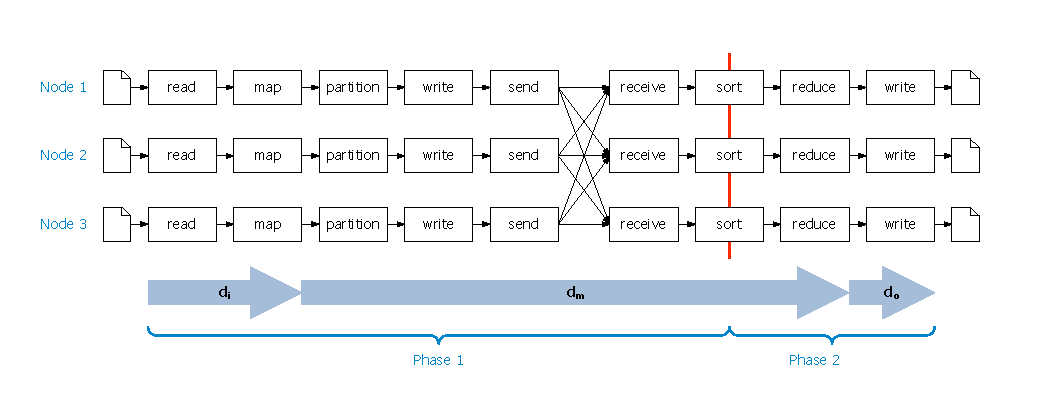
\includegraphics[width=6in]{fig_mapreduce_dataflow.eps}
}

\end{center}
\minicaption{A map-reduce dataflow}

\label{fig:mapreduce}
\end{figure}
}


\minorsection{Phase 1}
Phase 1 begins with the reading of the input data from disk and ends with the
sort operator. It includes the map operators and the exchange of data over the
network.
The first write operator in Phase~1 stores the output of the map operator.
This ``backup write'' operator is optional, but used by default in the
Google and Hadoop implementations of map-reduce, serving to increase the
system's ability to cope with failures or other events that may occur later.

\minorsection{Phase 2}
Phase 2 begins with the sort operator and ends with the writing of the output
data to disk. In systems that replicate data across multiple nodes,
such as the GFS \cite{gfs} and HDFS \cite{hdfs} distributed file systems
used with MapReduce and Hadoop, respectively, the output data must be sent
to all other nodes that will store the data on their local disks.

\minorsection{Parallelism}
In Figure \ref{fig:mapreduce},
partitioned parallelism takes place on the vertical axis;
the input data is split between three nodes, and each operator
is, in fact, split into three sub-operators that each run on a different node.
Pipelined parallelism takes place on the horizontal axis;
each operator within a phase processes data units (e.g., records) as it
receives them, rather than waiting for them all to arrive, and passes data
units to the next operator as appropriate.
The only breaks in pipelined parallelism occur at the boundary between phases.
As shown, this boundary is the sort operator.
The sort operator can only produce its first output record after it has
received all of its input records, since the last input record received
might be the first in sorted order.
%May want to add citation to work eliminating barrier

\minorsection{Quantity of data flow}
Figure \ref{fig:mapreduce} also illustrates how the amount of data ``flowing''
through the system changes throughout the computation. The amount of input data
per node is $d_i$, and the amount of output data per node is $d_o$. The amount
of data per node produced by the map operator and consumed by the reduce
operator is $d_m$. In most applications, the amount of data flowing through the
system either remains the same or decreases (i.e., $d_i \ge d_m \ge d_o$). 
In general, the mapper will implement some form of select, filtering out
rows, and the reducer will perform aggregation.  This reduction in data across the stages can play a key
role in the overall performance of the computation.  Indeed, Google's
MapReduce includes ``combiner'' functions
%\footnote{To the extent that
% we model combiner functions it is in the amount of data the mapper's
% output}
to move some of the aggregation work to the map operators and, hence,
reduce the amount of data involved in the network exchange~\cite{mapreduce}.
Many map-reduce workloads resemble a ``grep''-like computation, in which the map operator decreases
the amount of data ($d_i \gg d_m$ and $d_m = d_o$).
In others, such as in a sort, neither the map nor the reduce
function decrease the amount of data ($d_i = d_m = d_o$).

%the read
%operator reads the data from
%disk as a stream, so each record that is read from disk can be immediately
%passed to the map operator, which can convert (i.e., ``map'') that record into
%zero or more records that are then passed to the partition operator, and so
%forth. In other words, the map operator does not need to wait for all of the
%input to be read from disk, and the partition operator does not need to wait
%for the map operator to finish operating on all of the records.

%\fix{Need to talk about the optional backup write here, so it makes
%sense later in the model.  I see some commented out info on that here...}

%Without this mechanism, all map tasks must be re-executed if a single
%reduce task stops running.
%When running a long computation on a large cluster, where it is
%likely that one of the tasks will stop running during the computation, it is a
%good idea to include this step.  However, if the total number of ``machine
%hours'' required for a computation is small, the performance benefit from
%omitting this step probably outweighs the cost of having to re-run the
%computation if one of the tasks stops running during the original
%computation.

\subsection{Related work}
\label{sec:related_work}

Concerns about the performance of map-reduce style systems emerged
from the parallel databases community, where similar data processing
tasks have been tackled by commercially available systems. In
particular, Stonebraker et al.\ compare Hadoop to a variety of DBMSs
and find that Hadoop can be up to 36x slower than a commercial
parallel DBMS~\cite{stonebraker-mr}.  In previous
work~\cite{efficiencymatters}, two of the authors of our paper pointed
out that many parallel systems (especially map-reduce systems, but
also other parallel systems) have focused almost exclusively on
absolute throughput and high-end scalability.  This focus, as the
authors quantify by back-of-the-envelope comparisons, has been at the
detriment of other worthwhile metrics.
%Another author of this
%paper describes the analytical model in~\cite{tshiranthesis}.

In perhaps the most relevant prior work, Wang et al.\ use simulation
to evaluate how certain design decisions (e.g., network layout and data
locality) will effect the performance of Hadoop
jobs~\cite{mr-simulation}.  Specifically, their MRPerf simulator
instantiates fake jobs, which impose fixed times (e.g., job startup)
and input-size dependent times (cycles/byte of compute) for the Hadoop
parameters under study. The fake jobs generate network traffic
(simulated with ns-2) and disk I/O (also simulated).  Using execution
characteristics accurately measured from small instances of Hadoop
jobs, MRPerf accurately predicts (to within 5-12\%) the performance
of larger clusters.  Although simulation techniques like MRPerf are
useful for exploring different designs, by relying on measurements of
actual behavior (e.g., of Hadoop) such simulations will also emulate any
inefficiencies particular to the specific implementation simulated.

%DISC~\cite{disc}

%Efficiency matters~\cite{efficiencymatters} and Tomer's thesis~\cite{tshiranthesis}.

%MapReduce~\cite{mapreduce}, GFS~\cite{gfs}, Hadoop~\cite{hadoop}, HDFS~\cite{hdfs}, Dryad~\cite{dryad}.

%The language integration and translation to an execution plan has an
%effect on performance~\cite{distagg}.  Dryad LINQ~\cite{dryadlinq} and
%Pig latin~\cite{piglatin} provide higher-level SQL-like languages for
%expressing and automatically optimizing programs on a given system.

%DataSeries~\cite{dataseries} and Sawzall~\cite{sawzall}.

%Gordon~\cite{gordon} and FAWN~\cite{fawn}.

%Parallel database systems~\cite{paralleldatabases}, and Phoenix~\cite{phoenix}.

%Raid~\cite{raid}

\section{Performance model}
\label{sec:model}

This section presents a model for the runtime of a map-reduce job on a
hardware-efficient system.  It includes the model's assumptions,
parameters, and equations, along with a description of common
workloads.

\minorsection{Assumptions}
For a large class of data-intensive workloads, which we assume for our
model, computation time is negligible in comparison to I/O speeds.
Among others, this assumption holds for grep- and sort-like jobs, such
as those described by Dean and Ghemawat~\cite{mapreduce} as being
representative of most MapReduce jobs at Google, but may not hold in
other settings.
For workloads fitting the assumption, pipelined parallelism can allow
non-I/O operations to execute entirely in parallel with I/O operations,
such that overall throughput for each phase will be determined by the
I/O resource (network or storage) with the lowest effective throughput.
%In the absence of computationally expensive map or reduce
%tasks, we have observed that the I/O operators process data much
%slower than the CPU, so that the CPU is not the bottleneck.

For modeling purposes, we also do not consider specific network
topologies or technologies, and we assume that the network core is
over-provisioned enough that the internal network topology does not
impact the speeds of inter-node data transfers.  From our experience,
unlimited backplane bandwidth without any performance degradation is
probably impractical, although it was not an issue for our experiments
and we currently have no evidence for it causing issues on the other
large clusters which we analyze in Section~\ref{sec:discussion}.

The model assumes that input data is evenly distributed across all
participating nodes in the cluster, that nodes are homogeneous, and
that each node retrieves its initial input from local storage.  Most
map-reduce systems are designed to fit these assumptions.
\nocite{tashilocationaware} The model also accounts for output data
replication, assuming the common strategy of storing the first replica
on the local disks and sending the others over the network to other
nodes.  Finally, another important assumption is that a single job has
full access to the cluster at a time, with no competing jobs or other
activities.  Production map-reduce clusters may be shared by more than
one simultaneous job, but understanding a single job's performance is
a useful starting point.

%A common strategy that balances performance and reliability for 3-way
%replication is to store the first replica locally, the second replica
%on a different node of the same rack, and the third replica on a
%random node of a different rack.


\minorsection{Deriving the model from I/O operations}
Table~\ref{table:operations2} identifies the I/O operations in each
map-reduce phase for two variants of the sort operator.  When the data
fits in memory, a fast {\it in-memory sort} can be used. When it does
not fit, an {\it external sort} is used, which involves sorting each
batch of data in memory, writing it out to disk, and then reading and
merging the sorted batches into one sorted stream. The $\frac{n-1}{n}
d_m$ term appears in the equation, where $n$ is the number of nodes,
because in a well-balanced system each node partitions and transfers
that fraction of its mapped data over the network, keeping
$\frac{1}{n}$ of the data for itself.

{
\renewcommand{\baselinestretch}{1.0}
\begin{table}[t]
\centering
\begin{minipage}{1\textwidth}
\centering
\renewcommand{\arraystretch}{1.2}
\begin{tabular}{|l|l|l|}
\hline
        & $d_m < $ memory (in-memory sort) & $d_m \gg $ memory (external sort) \\ \hline
Phase 1
        & Disk read (input): $d_i$        & Disk read (input): $d_i$ \\
        & Disk write (backup): $d_m$      & Disk write (backup): $d_m$ \\
        & Network: $\frac{n-1}{n} d_m$    & Network: $\frac{n-1}{n} d_m$ \\
        &                                 & Disk write (sort): $d_m$ \\ \hline
Phase 2 & Network: $\left(r-1\right) d_o$ & Disk read (sort): $d_m$ \\
        &                                 & Network: $\left(r-1\right) d_o$ \\
        & Disk write (output): $r d_o$    & Disk write (output): $r d_o$ \\
\hline
\end{tabular}
\caption{I/O operations in a map-reduce job.
The first disk write in Phase 1 is an optional backup to protect
against failures.}
\label{table:operations2}
\end{minipage}
\end{table}
}


%NOTE: 4~GB sorts take up to 2.5 seconds on our cluster, so I had to
%take this out
%---on our four-core nodes, sorting 10 million 100-byte
%records takes only 0.3~seconds, which is a throughput of over 3~GB/s.

Table~\ref{table:symbols} lists the I/O speed and workload property
parameters of the model.
They include
%any replication factor used for the data output, and
%alternatives for describing the
amounts of data flowing through the system, which
%time, as altered by the map and reduce operations.  Those amounts can
%either be described
can be expressed either in absolute terms ($d_i$, $d_m$, and $d_o$) or in
terms of the ratios of the map and reduce operators' output and
input ($e_M$ and $e_R$, respectively).

{
\renewcommand{\baselinestretch}{1.0}
\begin{table}[t]
\centering
\begin{minipage}{1\textwidth}
\centering
\renewcommand{\arraystretch}{1.2}
\begin{tabular}{|l|p{13cm}|}
\hline
Symbol & Definition \\ \hline
$n$    & The number of nodes in the cluster. \\ \hline
$D_w$    & The aggregate disk \emph{write} throughput of a single node. A node with four disks, where each disk provides 65 MB/s writes, would have $D$ = 260
MB/s.
%\footnote{Disk speeds depend on the actual filesystem, the placement of blocks on the disks' tracks, and whether it is a write or a read.  
%Therefore, as discussed in Section~\ref{sec:optimality}, 
%we prefer to obtain these values empirically when possible. In our experiments, even when correcting for block placement to be in the fastest zone and using the faster \texttt{xfs} filesystem, write speeds lagged the raw device read throughput by 6-14\%.}
\\ \hline 
$D_r$    & The aggregate disk \emph{read} throughput of a single node. \\ \hline
$N$ & The network throughput of a single node.
% After accounting for unavoidable overhead, Gigabit Ethernet provides roughly $N$ = 110 MB/s.
\\ \hline 
$r$    & The replication factor used for the job's output data.  If no replication is used, $r=1$.  \\ \hline
$i$    & The total amount of input data for a given computation. \\ \hline
$d_i \left(= \frac{i}{n}\right)$  & The amount of input data per node, for a given computation. \\ \hline 
$d_m \left(= \frac{i \cdot e_M}{n}\right)$  & The amount of data per node after
the map operator, for a given computation. \\ \hline
$d_o \left(= \frac{i \cdot e_M \cdot e_R}{n}\right)$  & The amount of output
data per node, for a given computation. \\ \hline
$e_M \left(= \frac{d_m}{d_i}\right)$  & The ratio between the map operator's output and its input. \\ \hline
$e_R \left(= \frac{d_o}{d_m}\right)$  & The ratio between the reduce operator's output and its input.\\ \hline
\end{tabular}
\caption{Modeling parameters that include I/O speeds and workload properties.}
\label{table:symbols}
\end{minipage}
\end{table}
}


%Then, using the I/O operation patterns and modeling parameters, we derive our
Table~\ref{table:model:replication} gives the
model equations for the execution time of a map-reduce job
in each of four scenarios, representing the cross-product of the
Phase~1 backup write option ({\it yes} or {\it no}) and the sort type
({\it in-memory} or {\it external}).
In each case, the per-byte time to complete each phase (map and reduce)
is determined, summed, and multiplied by the number of input bytes per
node $\left(\frac{i}{n}\right)$.
The per-byte value for each phase is the larger (max) of that phase's
per-byte disk time and per-byte network time.
Using the last row (external sort, with backup write) as an example,
the map phase includes three disk transfers and one network transfer:
reading each input byte $\left(\frac{1}{D_r}\right)$, writing the $e_M$ map output
bytes to disk (the backup write; $\frac{e_M}{D_w}$),
writing $e_M$ bytes as part of the external sort $\left(\frac{e_M}{D_w}\right)$,
and sending $\frac{n-1}{n}$ of the $e_M$ map output bytes over the
network $\left(\frac{\frac{n-1}{n} e_M}{N}\right)$ to other reduce nodes.
The corresponding reduce phase includes two disk transfers and one
network transfer: reading sorted batches $\left(\frac{e_M}{D_r}\right)$,
writing $e_M e_R$ reduce output bytes produced locally $\left(\frac{e_M e_R}{D_w}\right)$
and $(r-1) e_M e_R$ bytes replicated from other nodes $\left(\frac{(r-1) e_M e_R}{D_w}\right)$,
and sending $e_M e_R$ bytes produced locally to $(r-1)$ other nodes
$\left(\frac{e_M e_R \left(r - 1\right)}{N}\right)$.
Putting all of this together produces the equation shown.


%{
\renewcommand{\baselinestretch}{1.0}
\begin{table*}
\centering
\renewcommand{\arraystretch}{1.2}
\begin{tabular}{|l|l|l|}
\hline
& $d_m < memory$ & $d_m \gg memory$ \\ \hline
Without backup write & $max\left\{\frac{d_i}{D_r},
\frac{\frac{n-1}{n} d_m}{N}\right\} + \frac{d_o}{D_w}$ & 
$max\left\{\frac{d_i}{D_r} + \frac{d_m}{D_w}, \frac{\frac{n-1}{n} d_m}{N}\right\} + \frac{d_m}{D_r} + \frac{d_o}{D_w}$ \\ \hline
With backup write & $max\left\{\frac{d_i}{D_r} + \frac{d_m}{D_w}, \frac{\frac{n-1}{n} d_m}{N}\right\} + \frac{d_o}{D_w}$ & $max\left\{\frac{d_i}{D_r} + \frac{2 d_m}{D_w},
\frac{\frac{n-1}{n} d_m}{N}\right\} + \frac{d_m}{D_r} + \frac{d_o}{D_w}$ \\ \hline
\end{tabular}
\caption{The execution time of a map-reduce computation on a parallel dataflow system.}
\label{table:model:simple}
\end{table*}
}

{
\renewcommand{\baselinestretch}{1.0}
\begin{table*}
\centering
\renewcommand{\arraystretch}{1.2}
\begin{tabular}{|l|l|l|}
\hline
& $d_m < memory$ (in-memory sort) \\ \hline
Without backup write &
$\frac{i}{n} \left( max\left\{\frac{1}{D_r}, \frac{\frac{n-1}{n} e_M}{N}\right\} +
max\left\{\frac{r e_M e_R}{D_w}, \frac{e_M e_R \left(r - 1\right)}{N}\right\} \right)$ \\ \hline
With backup write & $\frac{i}{n} \left( max\left\{\frac{1}{D_r} + \frac{e_M}{D_w},
\frac{\frac{n-1}{n} e_M}{N}\right\} + max\left\{\frac{r e_M e_R}{D_w}, \frac{e_M
e_R \left(r - 1\right)}{N}\right\} \right)$ \\ \hline

& $d_m \gg memory$ (external sort) \\ \hline
Without backup write & $\frac{i}{n} \left( max\left\{\frac{1}{D_r} + \frac{e_M}{D_w},
\frac{\frac{n-1}{n} e_M}{N}\right\} + max\left\{\frac{e_M}{D_r} + \frac{r e_M e_R}{D_w},
\frac{e_M e_R \left(r - 1\right)}{N}\right\} \right)$ \\ \hline
With backup write & $\frac{i}{n} \left(
max\left\{\frac{1}{D_r} + \frac{2 e_M}{D_w}, \frac{\frac{n-1}{n} e_M}{N}\right\} +
max\left\{\frac{e_M}{D_r} + \frac{r e_M e_R}{D_w}, \frac{e_M e_R \left(r -
1\right)}{N}\right\} \right)$ \\ \hline

\end{tabular}
\caption{Model equations for the execution time of a map-reduce computation on a parallel dataflow system.
%, as a function of the total amount of input data ($i$) and the map-reduce data expansion ratios ($e_M$ and $e_R$), where output data is replicated across $r$ nodes
}
\label{table:model:replication}
\end{table*}
}


\minorsection{Applying the model to common workloads}
Many workloads benefit from a parallel dataflow system because they run
on massive datasets, either extracting and processing a small amount of
interesting data or shuffling data from one representation to another.
%Data transfers
%can be on the order of Petabytes or Terabytes, as many blocks of data
%(each of 64 MB by default in Hadoop, but sometimes larger) are read
%from disk, processed, and transferred over the network.
We focus on parallel sort and grep in analyzing systems and validating
our model, which Dean and Ghemawat~\cite{mapreduce} indicate
are representative of most programs written by users of Google's
MapReduce.

For a grep-like job that selects a very small
fraction of the input data, $e_M \approx 0$ and $e_R = 1$, meaning
that only a negligible amount of data is (optionally) written to the
backup files, sent over the network, and written to the output files.
Thus, the best-case runtime is determined by the initial input disk
reads:

\begin{equation}
t_{\textstyle grep} = \frac{i}{n D_r}
\label{eqn:grepmodel}
\end{equation}

A sort workload maintains the same amount of data in both the map and
reduce phases, so $e_M = e_R = 1$.  If the amount of data
per node is small enough to accommodate an in-memory sort and not
warrant a Phase~1 backup, the top equation of
Table~\ref{table:model:replication} is used, simplifying to:

\begin{equation}
t_{\textstyle sort} = \frac{i}{n}
\left( max\left\{\frac{1}{D_r}, \frac{n-1}{n N}\right\}
+ max\left\{\frac{r}{D_w}, \frac{r-1}{N}\right\} \right)
\label{eqn:sortmodel2}
\end{equation}


\minorsection{Determining input parameters for the model}
Appropriate parameter values are a crucial aspect of model accuracy,
whether using the model to evaluate how well a production system is
performing or to determine what should be expected from a hypothetical system.
%\minorsection{Configuration parameters}
The $n$ and $r$ parameters are system configuration choices that can
be applied directly in the model for both production and hypothetical
systems.

%\minorsection{Workload property parameters}
The amount of data flowing through various operators ($d_i$,
$d_m$, or $d_o$) depend upon the characteristics of the map and
reduce operators and of the data itself.  For a production system,
they can be measured and then plugged into a model that evaluates the
performance of a given workload run on that system.  For a
hypothetical system, or if actual system measurements are not
available, some estimates must be used, such as $d_i = d_m = d_o$ for
sort or $d_m = d_o = 0$ for grep.

The determination of which equation to use, based on the backup write
option and sort type choices, is also largely dependent on the
workload characteristics, but in combination with system
characteristics.  Specifically, the sort type choice depends on the
relationship between $d_m$ and the amount of main memory available for
the sort operator.  The backup write option is a softer choice, worthy
of further study, involving the time to do a backup write
$\left(\frac{d_m}{D_w}\right)$, the total execution time of the job,
and the likelihood of a node failure during the job's execution.  Both
Hadoop and Google's MapReduce always do the backup write, at least to
the local file system cache.

%\minorsection{I/O speed parameters}
The appropriate values for I/O speed depend on what is being evaluated.
For both production and hypothetical systems, specification values
for the hardware can be used---for example, 1~Gbps for the network
and the maximum streaming bandwidth specified for the given disk(s).
This approach is appropriate for evaluating the efficiency of the
entire software stack, from the operating system up.
However, if the focus is on the programming framework, using raw
hardware specifications can indicate greater inefficiency than is
actually present.
In particular, some efficiency is generally lost in the underlying
operating system's conversion of raw disk and network resources into
higher level abstractions, such as file systems and network sockets.
To focus attention on programming framework inefficiencies,
one should use measurements of the disk and network bandwidths available
to applications using the abstractions.
As shown in our experiments, such measured values are lower than
specified values and often have non-trivial characteristics, such as
dependence on file system age or network communication patterns.
%In our evaluations of existing systems, we discuss both approaches.


\section{Existing data-intensive computing systems are far from optimal}
\label{sec:benchmarks}

%Published terasort and petasort benchmarks indicate 3-16x longer sort times compared to the optimal performance model.  It includes a results for Grep and TeraSort benchmarks in Figure~\ref{fig:benchmarks1}, results for PetaSort benchmarks in Figure~\ref{fig:benchmarks2}, a more complete listing of the configuration of each system, what our model predicts is the bottleneck resource, and how each system performed as compared to the optimal performance model.

%{
\renewcommand{\baselinestretch}{1.0}
\begin{figure}[t]
\begin{center}

%\resizebox{\columnwidth}{!} {
%   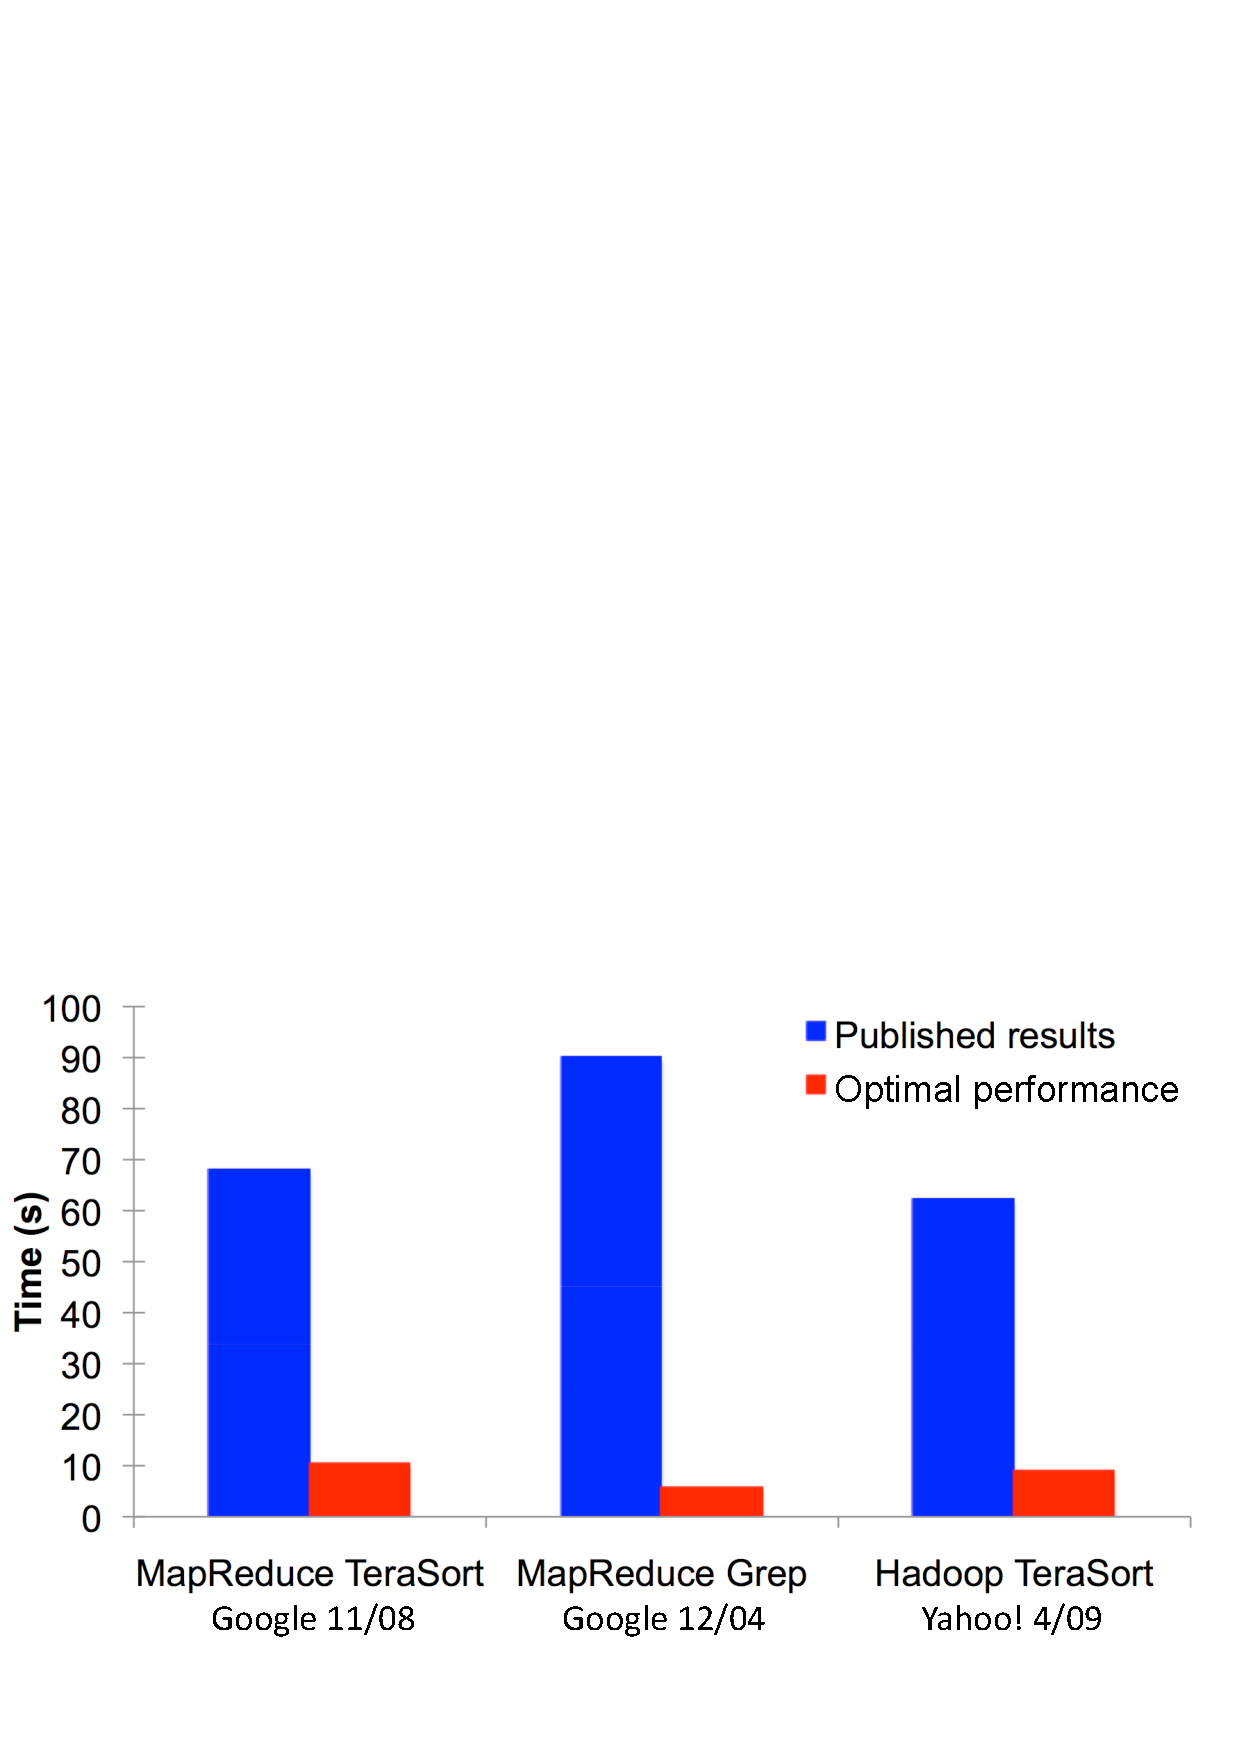
\includegraphics[height=2.5in]{fig_benchmarks1.pdf}
   
\includegraphics[height=2.5in]{pdllogo.eps}
%}

\end{center}
\minicaption{Published benchmarks for Grep and PetaSort}
{
}

\label{fig:benchmarks1}
\end{figure}
}


%
%{
\renewcommand{\baselinestretch}{1.0}
\begin{figure}[t]
\begin{center}

%\resizebox{\columnwidth}{!} {
%   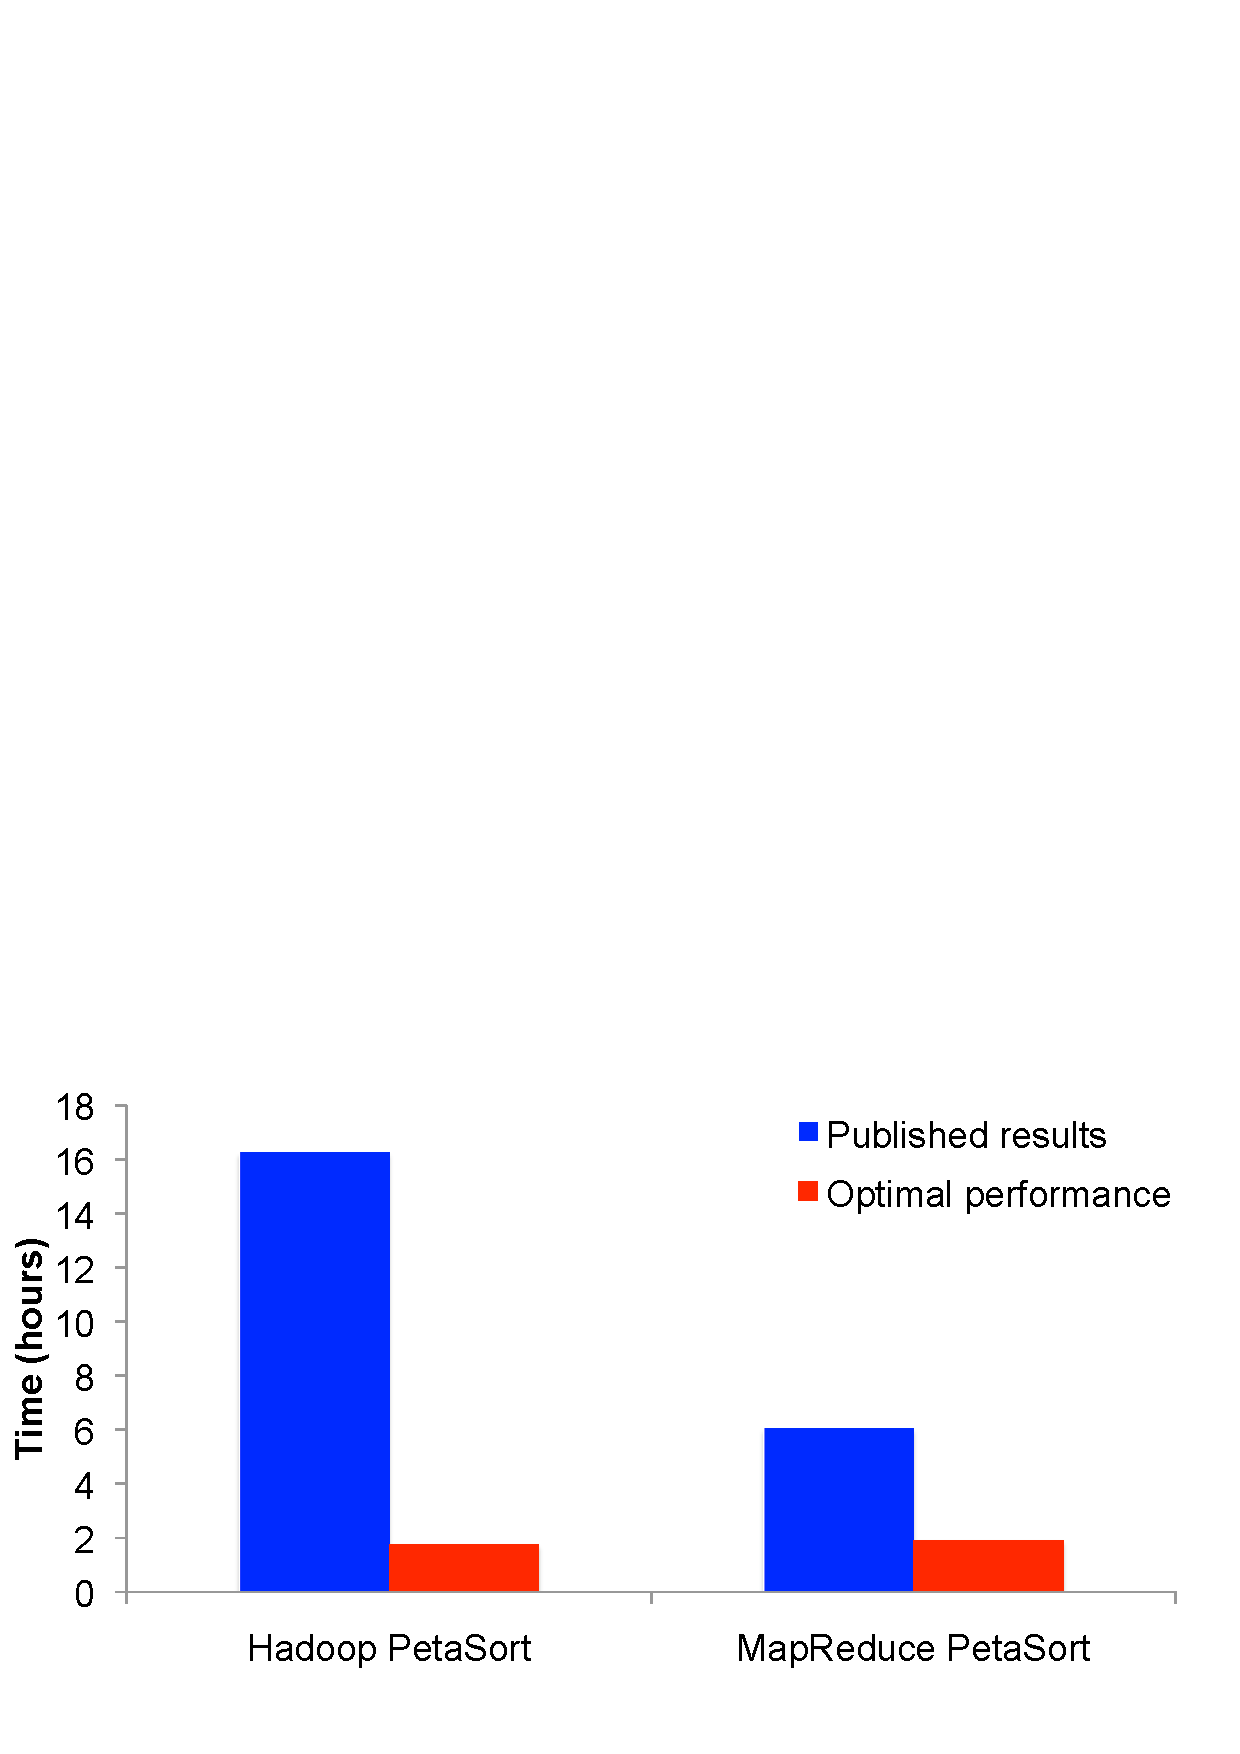
\includegraphics[height=2.5in]{fig_benchmarks2.pdf}
   
\includegraphics[height=2.5in]{pdllogo.eps}
%}

\end{center}
\minicaption{Published benchmarks for TeraSort}
{
}

\label{fig:benchmarks2}
\end{figure}
}




Our model indicates that, though they may scale beautifully, popular
data-intensive computing systems leave a lot to be desired in terms of
efficiency.  Figure~\ref{fig:slowdown} compares optimal times, as
predicted by the model, to reported measurements of a few benchmark
landmarks touted in the literature, presumably on well-tuned instances
of the programming frameworks utilized. These results indicate that
far more machines and disks are often employed than would be needed
if the systems were hardware-efficient.
The remainder of this section describes the systems and benchmarks
represented in Figure~\ref{fig:slowdown}.

%I removed mention of our own experiments on Hadoop for comparison,
%because I think the Hadoop results demonstrate that a lot of
%efficiency is lost at scale, so our 25-node hadoop
%performance isn't a good comparison point for these massive systems

{
\renewcommand{\baselinestretch}{1.0}
\begin{figure}[t]
\begin{center}

   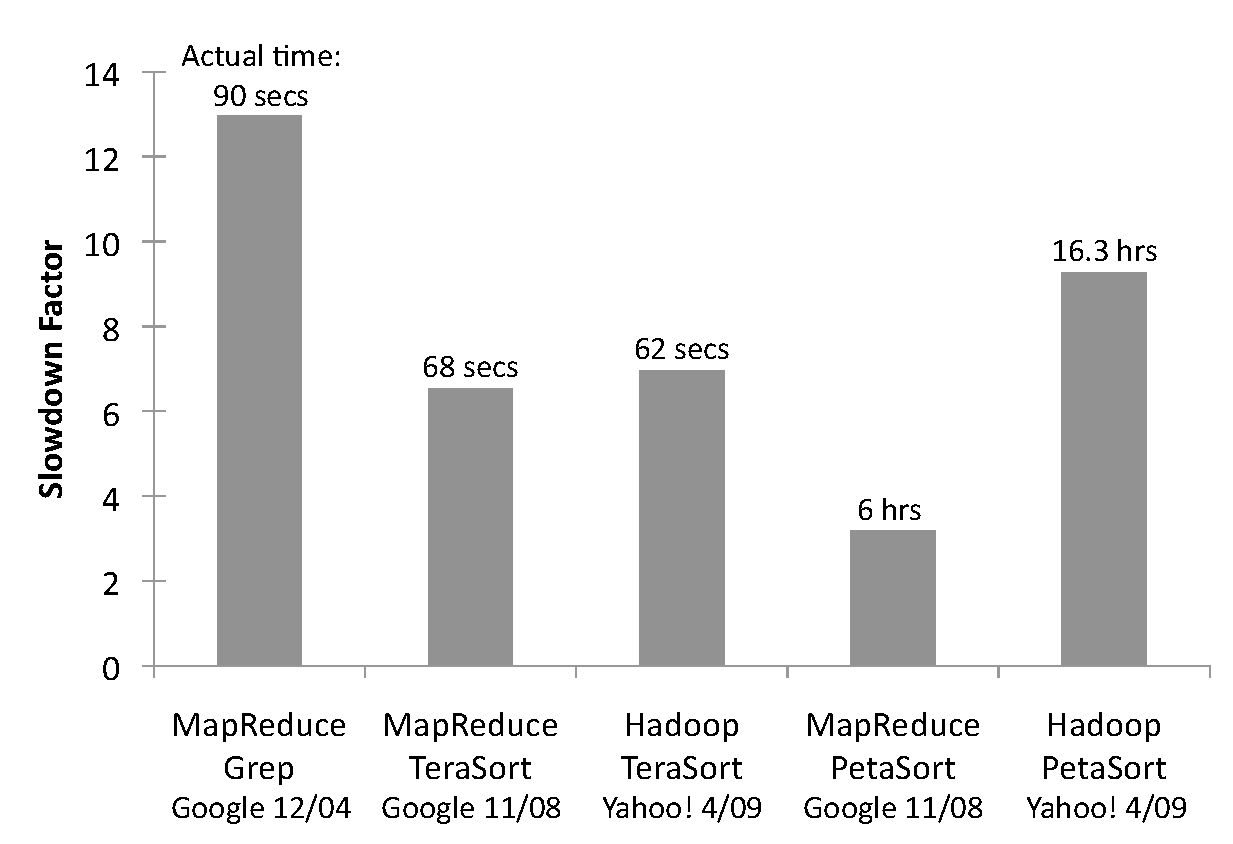
\includegraphics[height=2.5in]{fig_slowdown.eps}

\end{center}
\minicaption{Published benchmarks of popular parallel dataflow
  systems} {Each bar represents the reported throughput relative to
  the ideal throughput indicated by our performance model,
  parameterized according to a cluster's hardware.  }

\label{fig:slowdown}
\end{figure}
}



\minorsection{Hadoop -- TeraSort}
In April 2009,
Hadoop set a new record~\cite{hadoop2009} for sorting 1 TB of data in
the Sort Benchmark \cite{sortbenchmark} format.  The setup had the
following parameters: $i = 1$~TB, $r = 1$,
$n = 1460$, $D = 4$~disks~$\cdot 65$~MB/s/disk $= 260$~MB/s, $N = 110$~MB/s, $d_m = i/n = 685$~MB.
With only 685 MB per node, the data can be sorted by the individual nodes in
memory.
A phase~1 backup write is not needed, given the short runtime.
Equation~\ref{eqn:sortmodel2} gives a best-case runtime of 8.86~seconds.
%A backup write is not beneficial, in this case, so we can apply
%Equation \ref{eqn:sortmodel2} to obtain the optimal execution time:
%\[t_{\textstyle optimal} = \frac{1000000}{1460} \left( \frac{1}{110} + \frac{1}{260}
%\right) = 8.86 \textstyle{ seconds}\]
After fine-tuning the system for this specific
benchmark, Yahoo! achieved
% $t_{\textstyle actual} = 62$
62~seconds---$7\times$ slower.
% than the best-case runtime.
An optimal system using the same hardware would achieve better
throughput with 209 nodes (instead of 1460).

\minorsection{MapReduce -- TeraSort}
In November 2008,
Google reported TeraSort results for 1000 nodes with
12 disks per node~\cite{sorting1pb}. The following parameters were
used: $i = 1$~TB, $r = 1$, $n = 1000$, $D = 12 \cdot 65 = 780$~MB/s,
$N = 110$~MB/s, $d_m = i/n = 1000$~MB.
Equation~\ref{eqn:sortmodel2} gives a best-case runtime of 10.4~seconds.
%As with the Hadoop TeraSort, we can apply
%Equation~\ref{eqn:sortmodel2} to obtain the optimal execution time:
%\[t_{\textstyle optimal} = \frac{1000000}{1000} \left( \frac{1}{110} + \frac{1}{780}
%\right) = 10.37 \textstyle{ seconds}\]
Google achieved
% $t_{\textstyle actual} = 68$
68~seconds---over $6\times$ slower.
% than the best-case runtime.
An optimal system using the same hardware would achieve better
throughput with 153 nodes (instead of 1000).

\minorsection{MapReduce -- PetaSort}
Google's PetaSort experiment~\cite{sorting1pb} is similar to TeraSort,
with three differences:
(1) an external sort is required with a larger
amount of data per node ($d_m = 250$~GB),
(2) output was stored on GFS with three-way replication,
(3) a Phase~1 backup write is justified by the longer runtimes.
In fact, Google ran the experiment multiple times, and at least one disk
failed during each execution.
The setup is described as follows:
$i = 1$~PB, $r = 3$, $n = 4000$, $D = 12 \cdot 65 = 780$~MB/s,
$N = 110$~MB/s, $d_m = i/n = 250$~GB.
The bottom cell of Table~\ref{table:model:replication} gives
a best-case runtime of 6818~seconds.
%Referring to the bottom cell of Table \ref{table:model:replication}:
%\begin{equation}
%t_{\textstyle optimal}
%  = \frac{i}{n} \left( max\left\{\frac{3}{D},
%\frac{1}{N}\right\} + max\left\{\frac{4}{D}, \frac{2}{N}\right\} \right)\\
%%  = \frac{1000000000}{4000} \left( max\left\{\frac{3}{780},
%% \frac{1}{110}\right\} + max\left\{\frac{4}{780}, \frac{2}{110}\right\}
%% \right)\\
%= 6818 \textstyle{ seconds} 
%\end{equation}
Google achieved
% $t_{\textstyle actual} = 21720$
21,720~seconds---approximately $3.2\times$ slower.
% than the best-case runtime.
An optimal system using the same hardware would
achieve better throughput with 1256 nodes (instead of 4000).
Also, according to our model, for the purpose of sort-like
computations, Google's nodes are over-provisioned with disks. In an optimal
system, the network would be the bottleneck even if each node had only 6
disks instead of 12.

%FIXME: Add reasons for google over-provisioning?

\minorsection{Hadoop -- PetaSort}
Yahoo!'s PetaSort experiment~\cite{hadoop2009} is similar to Google's,
with one
difference: The output was stored on HDFS with two-way replication.
The setup is described as follows: $i = 1$~PB, $r = 2$, $n = 3658$, $D = 4 \cdot 65 = 260$~MB/s,
$N = 110$~MB/s, $d_m = i/n = 273$~GB.
The bottom cell of Table~\ref{table:model:replication} gives
a best-case runtime of 6308~seconds.
%\begin{equation}
%t_{\textstyle optimal} = \frac{i}{n} \left( max\left\{\frac{3}{D}, \frac{1}{N}\right\} + max\left\{\frac{3}{D}, \frac{1}{N}\right\} \right)\\
%%  = \frac{1000000000}{3658} \left( max\left\{\frac{3}{260}, \frac{1}{110}\right\} + max\left\{\frac{3}{260}, \frac{1}{110}\right\} \right)\\
%  = 6308.6 \textstyle{ seconds}
%\end{equation}
Yahoo! achieved
% $t_{\textstyle actual} = 58500$
58,500~seconds---about $9.3\times$
slower.
% than the best-case runtime.
An optimal system using the same hardware would achieve better
throughput with 400 nodes (instead of 3658).

\minorsection{MapReduce -- Grep}
The original MapReduce paper \cite{mapreduce} described a distributed grep
computation that was executed on MapReduce. The setup is described
as follows: $i = 1$~TB, $n = 1800$, $D = 2 \cdot 40 = 80$~MB/s,
$N = 110$~MB/s, $d_m = 9.2$~MB, $e_M = 9.2/1000000 \approx 0$, $e_R = 1$.
The paper does not specify the throughput of the disks, so we used 40 MB/s,
conservatively estimated based on disks of the timeframe (2004).
Equation \ref{eqn:grepmodel} gives a best-case runtime of 6.94~seconds.
%these parameters is:
%\[t_{\textstyle optimal} = \frac{i}{n D} = 5.56 \textstyle{ seconds}\]
Google achieved
% $t_{\textstyle actual} = 150$
150~seconds including startup overhead,
or 90~seconds without that overhead---still about $13\times$ slower.
% than the best-case runtime.
An optimal system using the same hardware would achieve better
throughput with 139 nodes (instead of 1800).
The 60-second startup time experienced by MapReduce on a
cluster of 1800 nodes would also have been much shorter on a
cluster of 139 nodes.


%\minorsection{MapReduce -- OLD HADOOP?}
%Elie had noted "older Hadoop TeraSort~\cite{hadoop2008}"... what do we
%know about it?

%\minorsection{MapReduce -- our Hadoop?}
%This may be going in the other section, but here's a placeholder just
%in case.

%ekrevat: moved sources of inefficiency into the discussion section

\section{Exploring the efficiency of data-intensive computing}
\label{sec:measure}

The model indicates that there is substantial inefficiency in popular
data-intensive computing systems.  The remainder of the paper reports
and analyzes results of experiments exploring such inefficiency.  This
section describes our cluster and quantifies efficiency lost to OS
functionality.  Section~\ref{sec:hadoop} confirms the Hadoop
inefficiency indicated in the benchmark analyses, and
Section~\ref{sec:pds} uses a stripped-down framework to validate that
the model's optimal runtimes can be approached.
Section~\ref{sec:discussion} discusses these results and ties together
our observations of the sources of inefficiency with opportunities for
future work in this area.


\minorsection{Experimental cluster}
%Our experiments were performed on CMU's OpenCirrus cluster.
Our experiments used 1--25 nodes of a cluster.
Each node is configured with two quad-core
Intel Xeon E5430 processors, four 1 TB Seagate Barracuda ES.2 SATA drives,
16 GB of RAM, and a Gigabit Ethernet link to a Force10 switch.
% and 1 24-port Arista 7124S head-end switch.
The I/O speeds indicated by the hardware specifications are
$N=1$~Gbps and $D_r = D_w = 108$~MB/s (for the outer-most disk zone).
All machines run the Linux 2.6.24 Xen kernel, but none of our
experiments were run in virtual machines---they were all run directly
on domain zero.
The kernel's default TCP implementation (TCP NewReno using up to 1500~byte
packets) was used.
Except where otherwise noted, the XFS file system was used to manage
a single one of the disks for every node in our experiments.


%\subsection{I/O bandwidths achieved atop the operating system}


\minorsection{Disk bandwidth for applications}
For sufficiently large or sequential disk
transfers, seek times have a negligible effect on performance; raw
disk bandwidth approaches the maximum transfer rate to/from
the disk media, which is dictated by the disk's rotation speed
and data-per-track values~\cite{Ruemmler94local}.
For modern disks, ``sufficiently large'' is on the order of
8~MB~\cite{Wachs07local}.
Most applications do not access the raw disk, instead accessing
the disk indirectly via a file system.
%Figure~\ref{fig:disk_measurements} presents measurements of read and
%write speeds for a few representative transfer sizes on our Seagate
%Barracuda drives.
Using the raw disk, we observe 108~MB/s, which is in line with the
specifications for our disks.
Nearly the same bandwidth (within 1\%) can be achieved for large
sequential file reads on \texttt{ext3} and XFS file systems.
For writes, our measurements indicate more interesting behavior.
Using the \texttt{dd} utility with the sync option, a 64~MB block size,
and input from the \texttt{/dev/zero} pseudo-device, we observe
steady-state write bandwidths of 84~MB/s and 102~MB/s, respectively.
When writing an amount of data less than or close to the file system
cache size, the reported bandwidth is up to another 10\% lower, since the file
system does not start writing the data to disk immediately; that is,
disk writing is not occurring during the early portion of the utility
runtime.

This difference between read and write bandwidths causes us to use
two values ($D_r$ and $D_w$) in the model; our original model used
one value for both.
%The fact that writes take longer than reads is not a surprise, since
%disks are more careful about positioning over a sector before
%modifying its physical state.
The difference is not due to the underlying disks, which have the
same media transfer rate for both reads and writes.
Rather, it is caused by file system decisions regarding coalescing
and ordering of write-backs, including the need to update metadata.
XFS and \texttt{ext3} both maintain a write-ahead log for data consistency,
which also induces some overhead on new data writes.
\texttt{ext3}'s relatively higher write penalty is likely caused by its
block allocator, which allocates one 4~KB block at a time, in contrast
to XFS's variable-length extent-based allocator.~\footnote{To address some of these
shortcomings, the \texttt{ext4} file system improves the design and
performance of \texttt{ext3} by adding, among other things,
multi-block allocations~\cite{Kumar08}.}

%We compare measurements of the raw partition, by
%writing directly to the device, to measurements taken with newly-built
%\texttt{ext3} and \texttt{xfs} filesystems on the first (outermost)
%zone of the disk.  These measurements were made using the \texttt{dd}
%utility with 64~MB block sizes and averaged over 10 runs.  The write
%experiments use data from \texttt{/dev/zero}, the read experiments
%immediately discard their data into \texttt{/dev/null}, and all
%experiments sync and free the linux buffer cache before every run.
%The potential speedup effects of the disk's write buffer are
%negligible because the buffer size is insignificant in comparison to
%the data transfer size.

%{
\renewcommand{\baselinestretch}{1.0}
\begin{figure}[t]
\begin{center}

%\resizebox{\columnwidth}{!} {
%   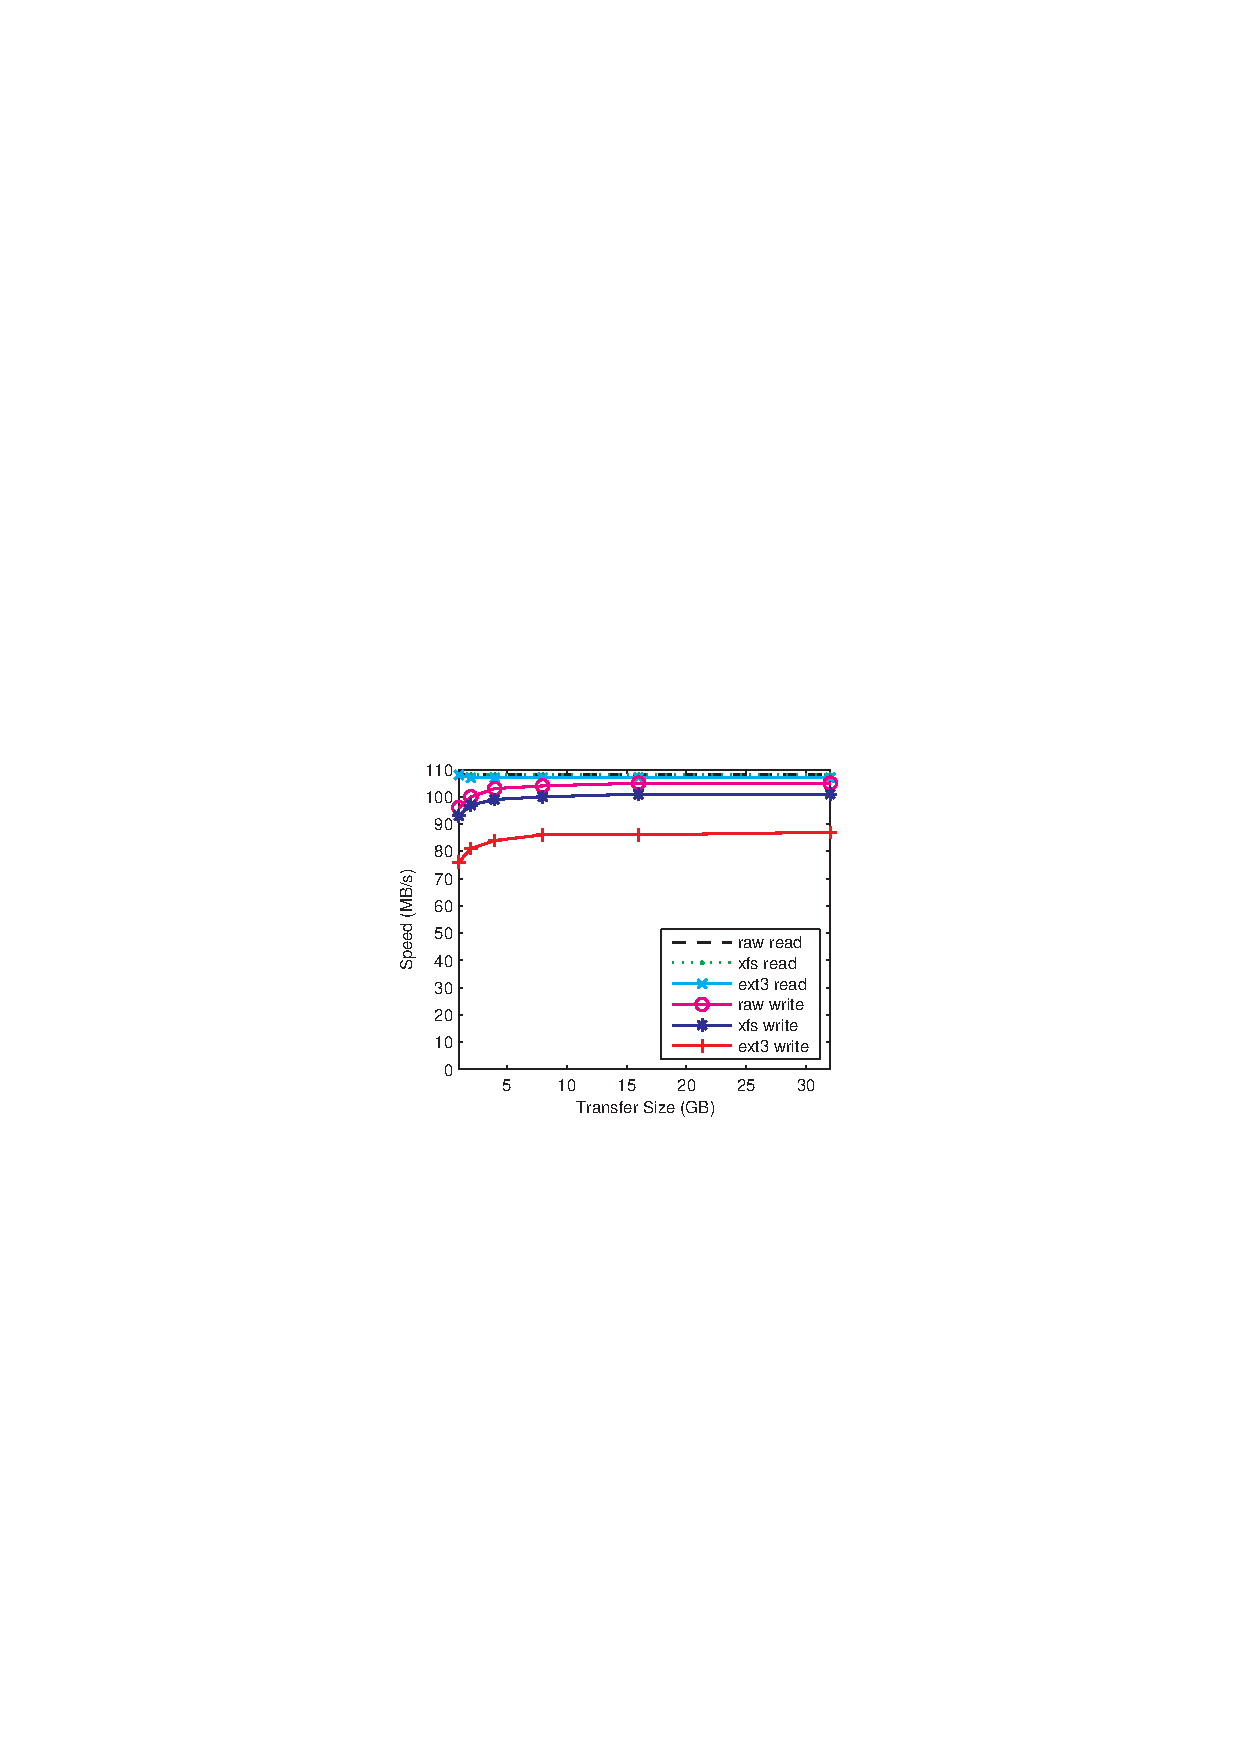
\includegraphics[height=2.5in]{fig_disk_measurements.pdf}
   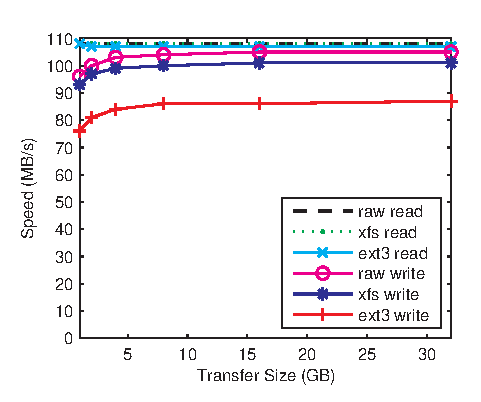
\includegraphics[height=2.5in]{fig_disk_measurements.eps}
%  }

\end{center}
\minicaption{Disk read and write measurements for a Seagate Barracuda drive}
{While read performance is consistently high across all systems,
  writes are slower, and \texttt{ext3} writes in particular are around
  20\% slower than raw device writes.}  

\label{fig:disk_measurements}
\end{figure}
}



%Our results show that Gigabyte-sized writes can be up to 32 MB/s
%slower than reads.  On the raw partition, this difference is smaller
%and becomes insignificant as the transfer size increases.  However, on
%ext3 and to a lesser extent on xfs, these differences become smaller
%but still persist for larger transfer sizes.

%Using the above results, we settled on XFS for use in all our
%subsequent experiments to get the fastest speeds, and a file size of
%4~GB per node to both achieve fast disk speeds and be able to keep all
%our intermediate data in memory.
The 108~MB/s value, and the \texttt{dd} measurements discussed above,
are for the first disk zone.
Modern disks have multiple zones, each with a different
data-per-track value and, thus, media transfer rate~\cite{Schindler02local}.
When measuring an XFS filesystem on a partition covering the entire disk,
read speeds remained consistent at 108 MB/s, but write speeds fluctuated
across a range of 92-102 MB/s with an average of 97 MB/s over 10 runs.
In reporting ``optimal'' values for experiments with our cluster, we
use 108~MB/s and 97~MB/s for the disk read and write speeds, respectively.

%However, these maximum transfer speeds also depend on the
%location of the data on disk -- the outer zones of a disk pack more
%sectors per track, allowing for faster data transfers than the zones
%that are closer to the spindle.

%Older, well-used filesystems may also be affected by fragmentation,
%which can interrupt sequential transfers with otherwise unnecessary
%disk seeks.  These issues can be solved by wiping and repartitioning
%the disks.  Therefore, we avoid dealing with fragmentation in our
%model.


\minorsection{Network bandwidth for applications}
Although a full-duplex 1~Gbps Ethernet link could theoretically
transfer 125~MB/s in each direction, maximum achievable data transfer
bandwidths are lower due to unavoidable protocol overheads.
Using the \texttt{iperf} tool with the maximum kernel-allowed 256~KB TCP
window size, we measured sustained bandwidths between two machines of
approximately 112.5 MB/s, which is in line with expected best-case
data bandwidth.
However, we observed lower bandwidths with more nodes in the all-to-all
pattern used in map-reduce jobs.
For example, in a 5--16 node all-to-all network transfer, we observed
102--106~MB/s aggregate node-to-node bandwidths over any one link.
These lower values are caused by NewReno's known slow convergence on
using full link bandwidths on high-speed networks~\cite{rapid-tcp}.
Such bandwidth reductions under some communication patterns may make
the use of a single network bandwidth ($N$) inappropriate for some environments.
For evaluating data-intensive computing on our cluster,
we use a conservative value of $N=110$~MB/s.

We also ran experiments using the newer CUBIC~\cite{cubic-tcp} congestion
control algorithm, which is the default on Linux 2.6.26 and is tuned to
support high-bandwidth links.
It achieved higher throughput (up to 115 MB/s per node with 10 nodes), but
exhibited significant unfairness between flows, yielding skews in
completion times of up to 86\% of the total time.
CUBIC's unfairness and stability issues are known and are prompting
continuing research toward better algorithms~\cite{rapid-tcp}.
%as a single speed.  However, since we do not have an implementation of
%better congestion control algorithms (e.g. RAPID~\cite{rapid-tcp}) for
%Linux, nor a more complex model that takes into account the high variability
%of NewReno and CUBIC, we use a conservative 110~MB/sec of network throughput
%with the understanding that we are overestimating the bandwidth achievable.

\section{Experiences with Hadoop}
\label{sec:hadoop}

We experimented with Hadoop on our cluster to confirm and better
understand the inefficiency exposed by our analysis of reported
benchmark results.
%and Section~\ref{sec:benchmarks}, we also measured the speed of Hadoop
%sorts on our cluster for up to 100 GB over 25 nodes.  We use weak
%scaling by keeping the amount of data per node constant and increasing
%the total amount of data to be sorted along with the active cluster size.


\minorsection{Tuning Hadoop's settings} Default Hadoop settings fail
to use most nodes in a cluster, using only two (total) map tasks and
one reduce task.  Even increasing those values to use four map and
reduce tasks per node, a better number for our cluster, with no
replication, still results in lower-than-expected performance.  We improved
the Hadoop sort performance by an additional 2$\times$ by adjusting a
number of configuration settings as suggested by Hadoop cluster setup
documentation and other
sources~\cite{hadoopsetup,hadoopsetup2,hadoopsetup3}.
%Initially we started with the
%default Hadoop settings, but by adjusting some key configurations we
%were able to improve sort times by a large factor. The actual number
%of possible settings and values were too large to do an exhaustive
%search, so there are certainly better settings and more changes to
%improve these Hadoop results even further.  However, these results
%represent our best efforts to adjust settings in ways commonly
Table~\ref{table:hadoop:settings} describes our changes, which
include reducing the replication level, increasing block sizes,
increasing the numbers of map and reduce tasks per node, and increasing
heap and buffer sizes.
%settings we changed to improve Hadoop's performance on our cluster,
%where one disk per node was made available to HDFS and up to 25 slave
%nodes (and one dedicated NameNode) were used for our experiments.
%First we changed the replication level from 3 to 1, to focus on the
%fastest case where replication is not necessary.  Larger block sizes
%helped our reads and writes go faster, and amortized the overhead for
%starting each map task.  We increased the maximum number of map and
%reduce tasks run in parallel per node, since our machines could handle
%the increased load.  We also increased the Java VM heap size, the
%Hadoop daemon heap size (used by each NameNode/DataNode and
%JobTracker/TaskTracker), the memory buffer sizes used for sorting, and
%the number of streams merged together when sorting.

Interestingly, we found that speculative execution did not improve
performance for our cluster.
Occasional map task failures and lagging nodes can
and do occur, especially when running over more nodes.
However, they are less common for our smaller cluster size
(one NameNode and 1--25 slave nodes), and surprisingly they
had little effect on the overall performance when they did occur.
%Add speculative execution citation from LATE paper in OSDI08?
When using speculative execution, it is generally
advised to set the number of total reduce tasks to 95---99\% of the
cluster's reduce capacity to allow for a node to fail and still
finish execution in a single wave.  Since failures are less of an
issue for our experiments, we optimized for the failure-free case and
chose enough Map and Reduce tasks for each job to fill every machine
at 100\% capacity.

{
\renewcommand{\baselinestretch}{1.0}
\begin{table}
\centering
\begin{minipage}{1\textwidth}
\centering
\renewcommand{\arraystretch}{1.2}
\begin{tabular}{|p{3.0cm}|c|c|p{9.4cm}|}
\hline
Hadoop Setting & Default & Tuned & Effect \\ \hline
Replication level & 3 & 1 & The replication level was set to 1 to
avoid extra disk writes. \\ \hline
HDFS block size & 64 MB & 128 MB & Larger block sizes in HDFS make large file reads and writes faster, amortizing the overhead for starting each map task. \\ \hline
Speculative exec. & $true$ & $false$ & Failures are uncommon on small clusters, avoid extra work. \\ \hline
Maximum map tasks per node  & 2 & 4 & Our nodes can handle more map
tasks in parallel. \\ \hline
Maximum reduce tasks per node & 1 & 4 & Our nodes can handle more
reduce tasks in parallel. \\ \hline
Map tasks & 2 & $4n$ & For a cluster of $n$ nodes, maximize the map tasks per node. \\ \hline
Reduce tasks & 1 & $4n$ & For a cluster of $n$ nodes, maximize the reduce tasks per node. \\ \hline
Java VM heap size & 200 MB & 1 GB & Increase the Java VM heap size for each child task. \\ \hline
Daemon heap size & 1 GB & 2 GB & Increase the heap size for Hadoop daemons. \\ \hline
Sort buffer memory & 100 MB & 600 MB & Use more buffer memory when sorting files.  \\ \hline
Sort streams factor & 10 & 30 & Merge more streams at once when sorting files. \\ \hline
\end{tabular}
\caption{Hadoop configuration settings used in our experiments.
%By tuning these Hadoop settings on our smaller cluster and running the specified maximum number of map and reduce tasks per node, our Hadoop sort benchmark completed about twice as fast as with the default Hadoop settings. While the actual default settings use 2 map tasks and 1 reduce task, that wouldn't actually make use of the full cluster of available machines.  Therefore, our modified default settings used a replication level of 1, $2n$ map tasks and $n$ reduce tasks.}
}
\label{table:hadoop:settings}
\end{minipage}
\end{table}
}


\minorsection{Sort measurements and comparison to the model}
\label{sec:hadoop:results}
Figure~\ref{fig:hadoopsort} shows sort results for different numbers
of nodes using our tuned Hadoop configuration.  Each measurement sorts
4~GB of data per node (up to 100~GB total over 25~nodes).  Random
100~byte input records were generated with the \emph{TeraGen} program,
spread across active nodes via HDFS, and sorted with the standard
\emph{TeraSort} Hadoop program.  Before every sort, the buffer cache
was flushed (with \texttt{sync}) to prevent previously cached writes
from interfering with the measurement.  Additionally, the buffer cache
was dropped from the kernel to force disk read operations for the
input data.  The sorted output is written to the file system, but not
synced to disk before completion is reported; thus, the reported
results are a conservative reflection of actual Hadoop sort execution
times.

{
\renewcommand{\baselinestretch}{1.0}
\begin{figure}[t]
\begin{center}
\subfigure[Scaling a Hadoop sort benchmark up to 25 nodes.]{
\includegraphics{fig_hadoop_sort.eps}
\label{fig:hadoopsort:scale}
}
\subfigure[Time breakdown into phases.]{
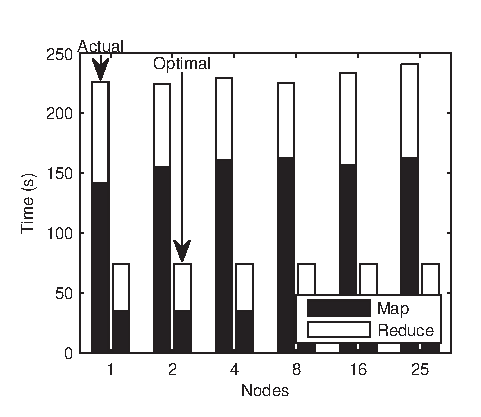
\includegraphics{fig_hadoop_breakdown.eps}
\label{fig:hadoopsort:breakdown}
}

\minicaption{Measured and optimal sort runtimes for a tuned Hadoop
  cluster.  Performance is about 3 times slower than optimal, and 2
  times slower than an optimal sort that includes an extra backup
  write for the map output, which is currently Hadoop's behavior}             
  {Hadoop scales well with 4~GB per node up to 25 nodes, but it is
  inefficient.  The measured runtime, optimal calculation, and optimal with
  backup write calculation are shown in {\bf (a)}.  The breakdown of
  runtime into map and reduce phases is shown in {\bf (b)}.

  % shows that a majority is spent in the map
  %, but there is considerable overhead
  %for creating and managing map and reduce tasks.  A breakdown
  %of the time in {\bf (b)} shows that a majority is spent in the map
  %phase, which includes time to setup the map and reduce tasks,
  %perform the map operation, and transfer data over the network to
  %the appropriate reducer. The reduce time includes the
  %actual sort and reduce operations, which will write the sorted data locally.}
}
\label{fig:hadoopsort}
\end{center}
\end{figure}
}



The results confirm that Hadoop scales well, since the average runtime
only increases 6\% (14 seconds) from 1 node up to 25 nodes (as the workload
increases in proportion).
For comparison, we also include the optimal sort times in
Figure~\ref{fig:hadoopsort}, calculated from our performance model.
The model's optimal values reveal a large constant inefficiency
for the tuned Hadoop setup---each sort requires 3$\times$ the optimal
runtime to complete, even without syncing the output data to disk.
%starting and managing map and reduce tasks is significant
%- 2 times longer than the predicted optimal times with an intermediate
%backup write, and 3 times longer without the backup write, which is
%unnecessary for our cluster.  If we hadn't tuned Hadoop beforehand,
%but instead used the default settings while being smart to maximize
%the number of map and reduce tasks per node and turn off replication,
%we discovered that it would have taken twice as long.  Put another
%way, tuning our Hadoop cluster from its default settings effectively
%doubled the efficiency of our cluster, but the sort still took 2 to 3
%times longer than an ideal system.

The 6\% higher total runtime at 25 nodes is due to skew in the completion
times of the nodes---this is the source of the $\sim$9\% additional
inefficiency at 25 nodes.
The inefficiency due to OS abstractions is already accounted for, as
discussed in Section~\ref{sec:measure}.
One potential explanation for part of the inefficiency is that Hadoop
uses a backup write for the map output, even though the runtimes are
short enough to make it of questionable merit.
As shown by the dotted
line in Figure~\ref{fig:hadoopsort}a, using the model equation with
a backup write would yield an optimal runtime that is 39~seconds longer.
This would explain approximately 25\% of the inefficiency.
However, as with the sort output, the backup write is sent to the file
system but not synced to disk---with 4~GB of map output per node
and 16~GB of memory per node, most of the backup write data may not
actually be written to disk during the map phase.
It is unclear what fraction of the potential 25\% is actually
explained by Hadoop's use of a backup write.

Another possible source of inefficiency could be unbalanced 
distribution of the input data or the reduce data.
%In terms of the actual workload matching up with the ideal of the
%model
However, we found that the input data is spread almost evenly across the
cluster.
Also, the difference between the ideal split of data and what is
actually sent to each reduce node is less than 3\%.
Therefore, the random input generation along with TeraSort's sampling and
splitting algorithms is partitioning work evenly,
and the workload distribution is not to blame
for the loss of efficiency.

Another potential source of inefficiency could be poor scheduling and task
assignment by Hadoop.
However, Hadoop actually did a good job at scheduling map tasks to run
on the nodes that store the data, allowing local disk access (rather
than network transfers) for over 95\% of the input data.
%The runs
%that had a higher percentage of local tasks was correlated with
%relatively shorter sort times, since less data had to be transferred
%over the network before it was processed.
The fact that this value was below 100\% is due to skew of
completion times where some nodes finish processing their local tasks
a little faster than others, and take over some of the load from the
slower nodes.

We do not yet have a full explanation for Hadoop's inefficiency.
Although we have not been able to verify in the complex Hadoop code,
some of the inefficiency appears to be caused by insufficiently pipelined
parallelism between operators, causing serialization of activities
(e.g., input read, CPU processing, and network write) that should
ideally proceed in parallel.
Part of the inefficiency is commonly attributed to CPU overhead
induced by Hadoop's Java-based implementation.
%Throughout each sort, each core running a map task was pegged at 100\%,
%despite the high-performance CPUs and low-CPU I/O-intensive task
%(reading and partitioning the data).
Of course, Hadoop may also not be using I/O resources at full efficiency.
More diagnosing of Hadoop's inefficiency is a topic for continuing
research.


\section{Verifying the model with Parallel DataSeries}
\label{sec:pds}

The Hadoop results above clearly diverge from the predicted optimal.
The large extent to which they diverge, however, brings the accuracy
of the model into question.  To validate our model, we present
Parallel DataSeries (PDS), a data analysis tool that attempts to
closely approach the maximum possible throughput.

\minorsection{PDS Design} Parallel DataSeries builds on DataSeries, an
efficient and flexible data format and runtime library optimized for
analyzing structured data~\cite{dataseries}.  DataSeries files are
stored as a sequence of \emph{extents}, where each extent is a series
of records.  The records themselves are typed, following a schema
defined for each extent.  Data is analyzed at the record level, but
I/O is performed at the much larger extent level.  DataSeries supports
passing records in a pipeline fashion through a series of modules.
PDS extends DataSeries with modules that support parallelism over
multiple cores (intra-node parallelism) and multiple nodes (inter-node
parallelism), to support parallel flows across modules as depicted in
Figure~\ref{fig:pds}.


{
\renewcommand{\baselinestretch}{1.0}
\begin{figure}[t]
\begin{center}

%\resizebox{\columnwidth}{!} {
%   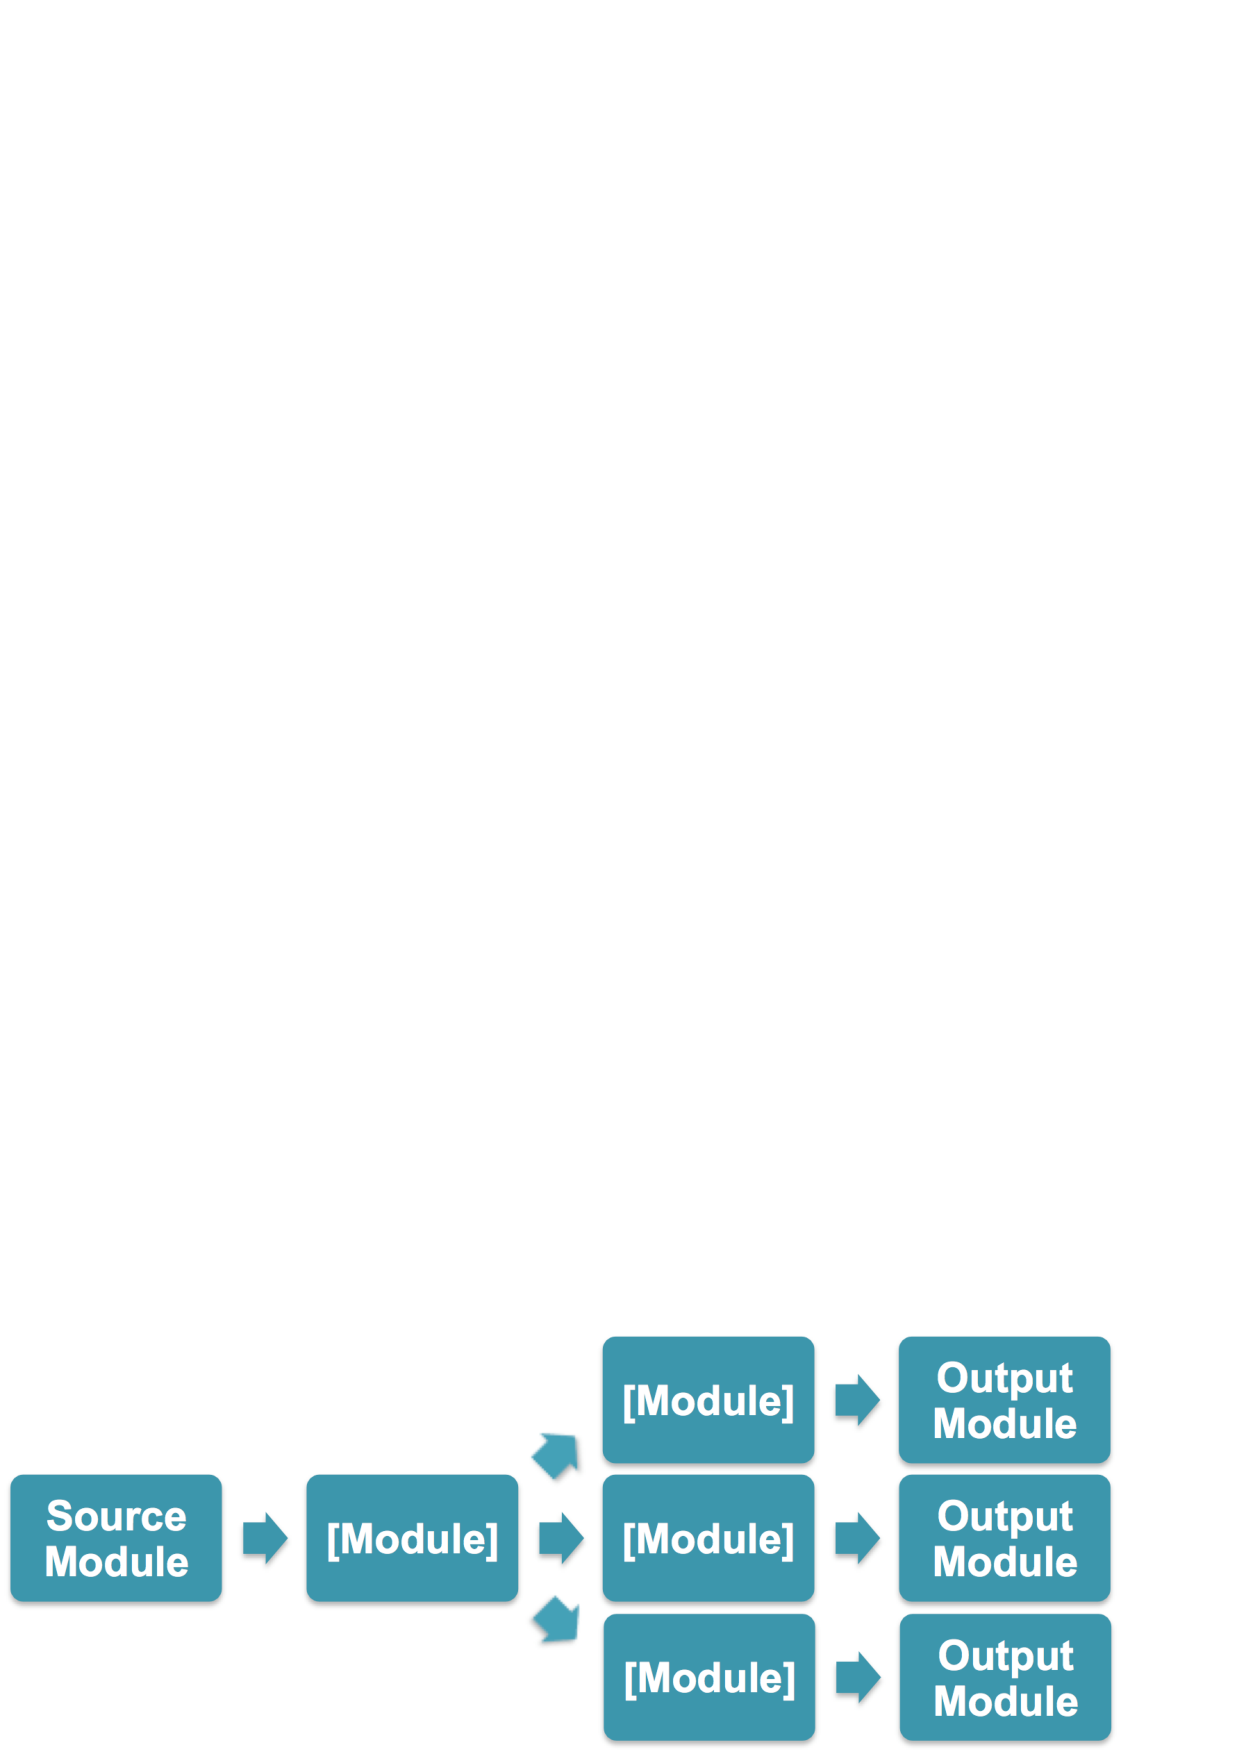
\includegraphics[height=1.5in]{fig_pds.pdf}
   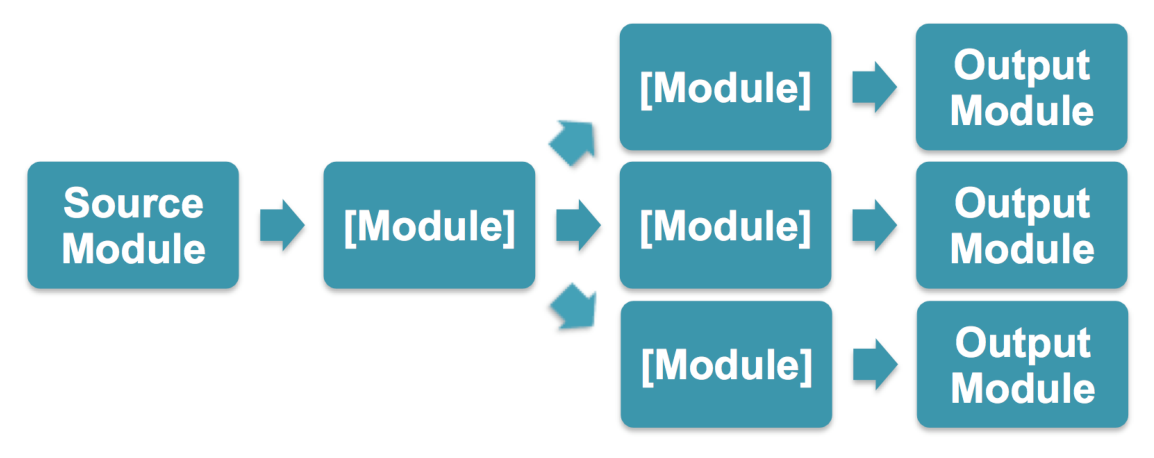
\includegraphics[height=1.5in]{fig_pds.eps}
%}

\end{center}
\minicaption{Parallel DataSeries is a carefully-tuned parallel runtime library for structured data analysis}
{Incoming data is queued and passed in a pipeline through a number of modules in parallel.}

\label{fig:pds}
\end{figure}
}



\minorsection{Sort evaluation} We built a parallel sort module in PDS
that implements a dataflow pattern similar to map-reduce.
In Phase 1, data is
partitioned and shuffled across the network.
As soon as a node receives all data from the shuffle, it exits Phase 1 and
begins Phase 2 with a local sort.  To generate input data for
experiments, we used
\emph{Gensort}, which is the sort benchmark~\cite{sortbenchmark} input generator
on which \emph{TeraGen} is based. The Gensort input set is
separated into partitions, one for each node.
PDS doesn't currently utilize a distributed filesystem, so we
manually partition the input, with 40 million records ($\sim$4 GB) at
each node.  We converted the GenSort data to DataSeries format without
compression, which expands the input by 4\%.
%note the 4 % cannot be from extent headers unless the extents are silly small.
%It is probably alignment overhead in the fixedwidth fields; 2 bytes for the 10 byte
%key (for 12 bytes total) and 2 bytes on the 90 byte record = 4 extra bytes per 100.

We measured PDS to see how closely it performed to the optimal
predicted performance on the same cluster used for the Hadoop
experiments.  Figure~\ref{fig:pds:sort1} presents the equivalent sort task
as run for Hadoop.  We repeated all experiments 10 times, starting
from a cold cache and syncing all data to disk before terminating the
measurement.
%reported, along with error bars for the measured standard deviation in
%each direction.  
As with the earlier Hadoop measurements, time is
broken down into each phase.  Furthermore, average per-node times are
included for the actual sort, as well as a \emph{stragglers} category
that represents the average wait time of a node from the time it
completes all its work until the the last node involved in the
parallel sort also finishes.

PDS performed well at 12-24\% of optimal.  About 4\% of that is the
aforementioned input expansion.  The sort time takes a little over 2
seconds, which accounts for another 3\% of the overhead.  Much of this
CPU could be overlapped with IO (PDS doesn't currently), and it is
sufficiently small to justify excluding CPU time from the model.
These two factors explain most of the 12\% overhead of the single node
case, leaving a small amount of natural coordination and runtime
overhead in the framework.  As the parallel sort is scaled to 25
nodes, besides the additional coordination overhead from code
structures that enable partitioning and parallelism, the remaining
divergence can be mostly explained by two factors: (1) straggler
nodes, and (2) network slowdown effects from many competing transfers.
Stragglers (broken out in Figure~\ref{fig:pds:sort1}b) can be the
result of generally slow (i.e., ``bad'') nodes, skew in network
transfers, or variance in disk write times.  The up to 5\% observed
straggler overhead is reasonable.  The network slowdown effects were
identified in Section~\ref{sec:measure} using \texttt{iperf}
measurements, and are mostly responsible for the slight time increase
starting around 4 nodes.  However, even if the effective network
goodput speeds were 100 MB/s instead of the 110 MB/s used with the
model, that would eliminate only 4\% of the additional overhead for
our PDS results compared to the predicted optimal time.  As more nodes
are added at scale, the straggler effects and network slowdowns become
more pronounced.

{
\renewcommand{\baselinestretch}{1.0}
\begin{figure}[t]
\begin{center}
\subfigure[Scaling a PDS sort benchmark up to 25 nodes.]{
\includegraphics{fig_pds_sort1.eps}
\label{fig:pds:sort1:scale}
}
\subfigure[Time breakdown.]{
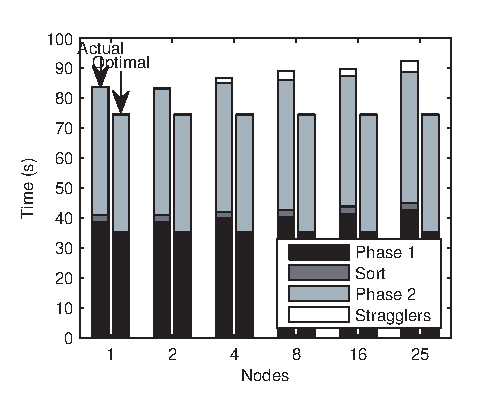
\includegraphics{fig_pds_breakdown1.eps}
\label{fig:pds:sort1:breakdown}
} \minicaption{Using Parallel DataSeries to sort up to 100~GB, it is
  possible to approach within 12-24\% of the optimal sort times as
  predicted by our performance model} {PDS scales well for an
  in-memory sort with 4~GB per node up to 25 nodes in {\bf (a)},
  although there is a small time increase starting around 4 nodes due
  to network effects.  Also shown for the 25 node case is the
  performance of our older, unbalanced partitioner, which had an
  additional 6\% performance overhead from optimal.  A breakdown of
  time in {\bf (b)} shows that the time increases at scale are mostly
  in the first phase of a map-reduce dataflow, which includes the
  network data shuffle, and in the time nodes spend waiting for
  stragglers due to effects of skew. }

\label{fig:pds:sort1}
\end{center}
\end{figure}
}



When we originally ran these experiments and inspected the results of
the 25 node case, we noticed that 6 of the nodes consistently finished
later and were processing about 10\% more work than the other 19.  It
turned out that our data partitioner was using only the first byte of
the key to split up the space into 256 bins, so it partitioned the
data unevenly for clusters that were not a power of 2.  After
designing a fairer partitioner that used more bytes of the key, and
applying it to the 25 node parallel sort, we were able to bring down
the overhead from 30\% to 24\%.

To see how both the model and PDS react to the network as a
bottleneck, we configured our network switches to negotiate 100 Mbps
Ethernet.  Just as the $\frac{n-1}{n} N$ term in the model predicts
increasingly longer sort times which converge in scale as more nodes
participate, Figure~\ref{fig:pds:sort2} demonstrates that our actual
results with PDS match up very well to that pattern.  The PDS sort
results vary between 12-27\% slower than optimal.
%FIXME waiting for new numbers to update this:
%with the same outlier at 25 nodes due to poor partitioning.  
For clusters of size 16 and 25, 5\% of the time is spent waiting for
stragglers. The slow speed of the network amplifies the effects of
skew; we observed a few nodes finishing their second phase before the
most delayed nodes had received all of their data from the first
phase.

{
\renewcommand{\baselinestretch}{1.0}
\begin{figure}[t]
\begin{center}
\subfigure[Scaling a PDS sort benchmark up to 25 nodes.]{
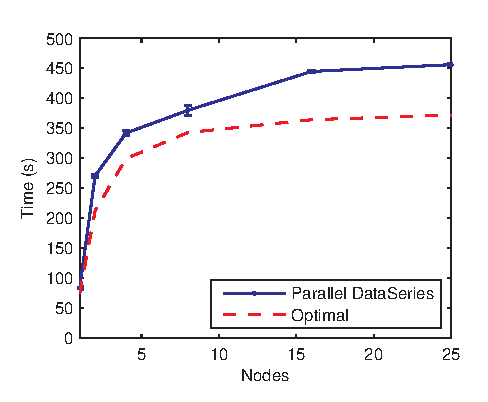
\includegraphics{fig_pds_sort2.eps}
\label{fig:pds:sort2:scale}
}
\subfigure[Time breakdown into phases.]{
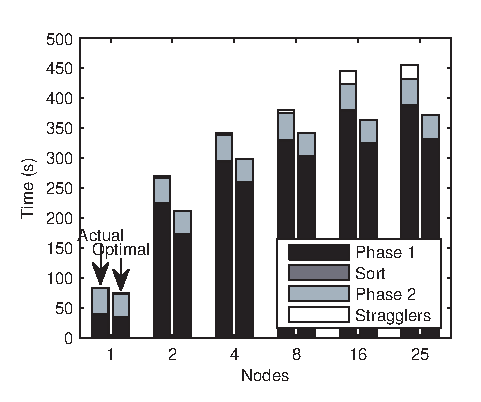
\includegraphics{fig_pds_breakdown2.eps}
\label{fig:pds:sort2:breakdown}
}
\minicaption{With 100~Mbps Ethernet as the bottleneck resource,
  a 100~GB sort benchmark on Parallel DataSeries matches up well with
  the model's prediction and stays within 12-27\% of optimal}
{As more data is sent over the network with larger cluster sizes in
  {\bf (a)}, both the model
  and PDS predict longer sort times that eventually converge.
  A breakdown of time in {\bf (b)} shows that the predicted and actual
  time increases occur during the first map-reduce phase, which
  includes the network data shuffle.}

\label{fig:pds:sort2}
\end{center}
\end{figure}
}



\section{Discussion}
\label{sec:discussion}

The experiments with PDS demonstrate that our model is not wildly
optimistic---it is possible to get close to the optimal runtime.
Thus, the inefficiencies indicated for our Hadoop cluster and the
published benchmark results are real.  We do not have complete
explanations for the 3--13$\times$ longer runtimes for current
data-intensive computing frameworks, but we have identified a number
of contributors.

One class of inefficiencies comes from duplication of work or
unnecessary use of a bottleneck resource.  For example, Hadoop and
Google's MapReduce always write phase~1 map output to the file system,
whether or not a backup write is warranted, and then read it from the
file system when sending it to the reducer node.  This file system
activity, which may translate into disk I/O, is unnecessary for
completing the job and inappropriate for shorter jobs.
%The disk read, at least, is unnecessary for completing the job,
%as is the write when backup is not needed.
%In addition, the I/O speed parameters ($N$, $D_r$, and $D_w$) used are
%the hardware specification values, so some portion of the efficiency
%is lost to OS abstractions---for example, the \fix{XXX}--YYY\% reported in
%Section~\ref{sec:measure} for our measured cluster.

One significant effect faced by map-reduce systems is that a job only
completes when the last node finishes its work.  For our cluster, we
analyzed the penalty induced by such stragglers, finding that it grows
to 4\% of the runtime for Hadoop over 25 nodes.  Thus, it is not the
source of most of the inefficiency at that scale.  For much larger
scale systems, such as the 1000+ node systems used for the benchmark
results, this straggler effect is expected to be much more
significant---it is possible that this effect explains much of the
difference between our measured 3$\times$ higher-than-optimal runtimes
and the published 6$\times$ higher-than-optimal runtime of the Hadoop
record-setting TeraSort benchmark.

The straggler effect is also why Google's MapReduce and Hadoop
dynamically distribute map and reduce tasks among nodes.  Support for
speculative execution also can help mitigate this effect, although
fault tolerance is its primary value.  If the straggler effect really
is the cause of poor end-to-end performance at scale, then it
motivates changes to these new data-parallel systems to examine and
adapt the load balancing techniques used in works like
River~\cite{river} or Flux~\cite{flux}.

It is tempting to blame lack of sufficient bisection bandwidth in the
network topology for much of the inefficiency at scale.  This would
exhibit itself as over-estimation of each node's true network
bandwidth, assuming uniform communication patterns, since the model
does not account for such a bottleneck.  However, this is not an issue
for the measured Hadoop results on our small-scale cluster because all
nodes are attached across two switches with sufficient backplane
bandwidth.  The network topology was not disclosed for most of the
published benchmarks, but for many we don't believe bisection
bandwidth was an issue.  For example, MapReduce grep involves minimal
data exchange because $e_M \approx 0$.  Also, for Hadoop PetaSort,
Yahoo! used 91~racks, each with 40~nodes, one switch, and an 8~Gbps
connection to a core switch (via 8~trunked 1~Gbps Ethernet links).
For this experiment, the average bandwidth per node was 4.7~MB/s.
% $\frac{1000000000/3658 \textstyle{MB}}{58500 s} = 4.7~MB/s.  Given
%that the vast majority of the network traffic ($90/91$) was between racks,
%racks,
Thus, the average bandwidth per uplink was only
%$90/91 \cdot 40 \cdot 4.67 = 184.87 \textstyle{MB/s} =
1.48~Gb/s in each direction, well below 8~Gbps.  Other
benchmarks may have involved a bisection bandwidth limitation, but
such an imbalance would have meant that far more machines were used
per rack (and overall) than were appropriate for the job, resulting in
significant wasted resources.

%For Hadoop, we have access to source code and can do our own experiments.
%Preliminary examination indicates substantial inefficiency induced 
%by its Java-based implementation and its componentized software architecture.
%The result is lack of streamlining and coordination across operators
%(e.g., inefficient dataflow) and across system layers (e.g.,
%between HDFS and Hadoop).
%XXX - this is generic... do we have anything that we can actually say?

Naturally, deep instrumentation and analysis of Hadoop will provide
more insight into its inefficiency.  Also, PDS in particular provides
a promising starting point for understanding the sources of
inefficiency.  For example, replacing the current manual data
distribution with a distributed file system is necessary for any
useful system.  Adding that feature to PDS, which is known to be
efficient, would allow one to quantify its incremental cost.  The same
approach can be taken with other features, such as dynamic task
distribution and fault tolerance.


\section{Conclusion}
\label{sec:conclusion}


Data-intensive computing is an increasingly popular style of computing
that is being served by scalable, but inefficient, systems.  A simple
model of optimal map-reduce job runtimes shows that popular map-reduce
systems take 3--13$\times$ longer to execute jobs than their hardware
resources should allow.  With Parallel DataSeries, our simplified
dataflow processing tool, we demonstrated that the model's runtimes
can be approached, validating the model and confirming the
inefficiency of Hadoop and Google's MapReduce.  Our model and results
highlight and begin to explain the inefficiency of existing systems,
providing insight into areas for continued improvements.

%Appropriately constructed, analytical models can be useful for more   
%than offline understanding of inefficiencies---they can be a critical 
%part of dynamic decision making in both operator selection within jobs
%and resource scheduling within the job management system.
%They can be used to avoid wasting over-provisioned resources by, for
%example, scaling down CPU speeds, turning off some disks, or adjusting
%the number of machines used for a job.
%They can also be used to decide whether to perform optional actions
%like backup writes of intermediate data that can
%be used to restart an interrupted job, rather than starting over.




{
\renewcommand{\baselinestretch}{1.0}
\small
\normalsize
\bibliography{local,submit}

%-- Bib style for citations of the form: [Zippy97]
%\bibliographystyle{$REFDIR/tex/macros/refalpha}

%-- Citations by number: [23]
%\bibliographystyle{$REFDIR/tex/macros/refplain}

%-- Citations by number w/ only the authors' 1st and middle initials
% We're including the local refabbrv so that the bibliography is generated
% even when REFDIR is not mounted.
% \bibliographystyle{$REFDIR/tex/macros/refabbrv}
\bibliographystyle{amsplain}
}

\end{document}

